% sage_latex_guidelines.tex V1.20, 14 January 2017
\documentclass[Afour,sageh,times]{sagej}

\usepackage{moreverb,url}
\usepackage[colorlinks,bookmarksopen,bookmarksnumbered,citecolor=red,urlcolor=red]{hyperref}
\usepackage{subfigure}
\usepackage{graphics} % for pdf, bitmapped graphics files
\usepackage{epsfig} % for postscript graphics files
\usepackage{mathptmx} % assumes new font selection scheme installed
\usepackage{times} % assumes new font selection scheme installed
\usepackage{amsmath} % assumes amsmath package installed
\usepackage{amssymb}  % assumes amsmath package installed
\usepackage{mathtools}
\usepackage{bm}
\usepackage{mathrsfs}
\usepackage{xcolor}
\usepackage{threeparttable}
\usepackage{multirow}
\usepackage{bigdelim}
\usepackage{algorithm}
\usepackage{algorithmicx}
\usepackage{algpseudocode}
\usepackage{graphicx}
\usepackage{comment}
\usepackage{galois}
\usepackage{array}

\newcommand\BibTeX{{\rmfamily B\kern-.05em \textsc{i\kern-.025em b}\kern-.08em
T\kern-.1667em\lower.7ex\hbox{E}\kern-.125emX}}

\def\volumeyear{-}

\setcounter{secnumdepth}{3}
\begin{document}

%\runninghead{Tong Yang \textit{et al.} Smooth Non-repetitive Manipulator Coverage with Minimal Discontinuities}
\runninghead{Tong Yang \textit{et al.} Least Discontinuity Non-revisiting Coverage Task with Smooth Transition to Valid Singularity}

%\title{Smooth Non-repetitive Manipulator Coverage with Minimal Discontinuities}
\title{Least Discontinuity Non-revisiting Coverage Task with Smooth Transition to Valid Singularity}

\author{Tong Yang\affilnum{1}, Jaime Valls Miro\affilnum{2}, Yue Wang\affilnum{1} and Rong Xiong\affilnum{1}}

\affiliation{\affilnum{1} State Key Laboratory of Industrial Control and Technology, Zhejiang University, P.R.China\\
\affilnum{2} Robotics Institute (UTS:RI), University of Technology Sydney, Sydney, Australia}

\corrauth{Yue Wang, wangyue@iipc.zju.edu.cn}%, Yuquan Campus, Zheda Road 38, Xihu District, Hangzhou, China}


\begin{abstract}
The Non-repetitive Coverage Path Planning (NCPP) is a crucial task carried out by manipulators in industrial applications. Nonlinear manipulator kinematics and the imposition of task-specified constraints dictate that applying conventional Coverage Path Planning (CPP) solutions on the target surface invariably result in truncated end-effector motions. 
On the other hand, coverage paths designed directly in joint-space cannot ensure reoccurrences will not arise. 
Without singularities, valid non-singular configurations only form disjoint sets which individually is injective to the target surface under kinematic mapping and is represented by a colour. 
\textcolor{blue}{Under such an assumption, previous works have modelled NCPP for non-redundant manipulators into a non-overlapping painting problem of a topological graph. }
However, singular configurations have been purposedly disregarded, hence invariably introducing end-effector lift-offs at such poses bridging the sets. 
Considering singular configurations violates the injectivity in the kinematic mapping - hence the definition of a single colour per configuration. 
This work however proves that by carefully choosing permissible paths considering the rank-deficient manipulability measure, valid singularities can be leveraged to further reduce the number of necessary end-effector discontinuities.
The scheme assumes a generic represention of surfaces as discrete meshes, symbolising a null probability to locate the point corresponding to valid but singular inverse kinematic solutions, and constructs a practical method to smoothly traverse a singularity without explicitly calculating it. 
Extensive simulated and realistic experiments are carried out for the examination of the proposed algorithm. 
\end{abstract}

\keywords{Optimal Cellular Decomposition, Non-repetitive Coverage Task, Singularity Analysis}

\maketitle

\section{Introduction}
Full coverage of the surface of a given object with non-redundant manipulators is embodied in tasks such as automatic polishing~\cite{Tian2016Polishing}, deburring~\cite{Xie2016Grinding}, painting~\cite{Li2011Painting} or surface inspection~\cite{Molina2017Defects}, where the need for non-repetitive coverage path planning (NCPP) is paramount to avoid over revisiting. 




The kinematic relationship of a typical manipulator makes mapping between task-space and joint-space non-bijective, which in effect drives coverage paths to be traditionally carried out in the former to ensure no revisiting of points in the surface~\cite{Oriolo2005Motion}. 
However, in further pursuing motions where the manipulator may minimise the number of reconfigurations is obliged to undertake to follow a desirable continuous end-effector (EE) path, a global optimal cellular decomposition problem in the joint-space has been 
proposed to incur joint-space partitions with minimum sets~\cite{Yang2020Cellular}~\cite{Yang2020Nonrevisiting}. 
This is illustrated in the example shown by Fig.~\ref{fig:TMech}: the external surface of a wok-like object is inspected by a non-redundant manipulator. 
Points on the surface can be reached by a variety of robot configurations. 
The three solid colour cells shown in Fig.~\ref{fig:TMech_config_cells} illustrate poses of disjoint sets reachable as a continuous set by a given configuration, \textcolor{blue}{such as ``shoulder-left \&  elbow-up \& wrist-unflipped" and ``shoulder-right \&  elbow-up \& wrist-flipped"}, visually seen by the different colours. 
\begin{figure}[t]
\centering
\subfigure[]{
	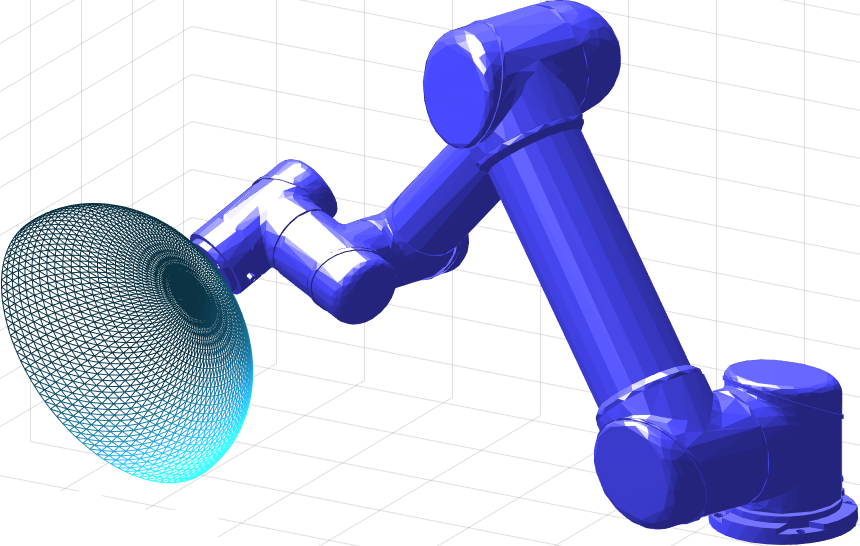
\includegraphics[width = 0.1\textwidth]{figures/TMech_simply_connected_example/design_demo_2}
	\label{fig:TMech_model}}
\subfigure[]{
	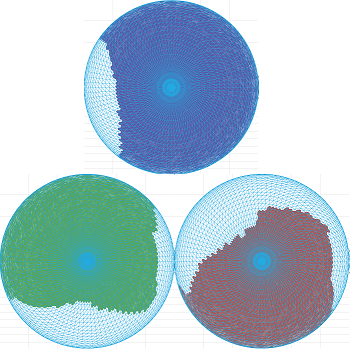
\includegraphics[width = 0.1\textwidth]{figures/TMech_simply_connected_example/design_comb}
	\label{fig:TMech_config_cells}}
\subfigure[]{
	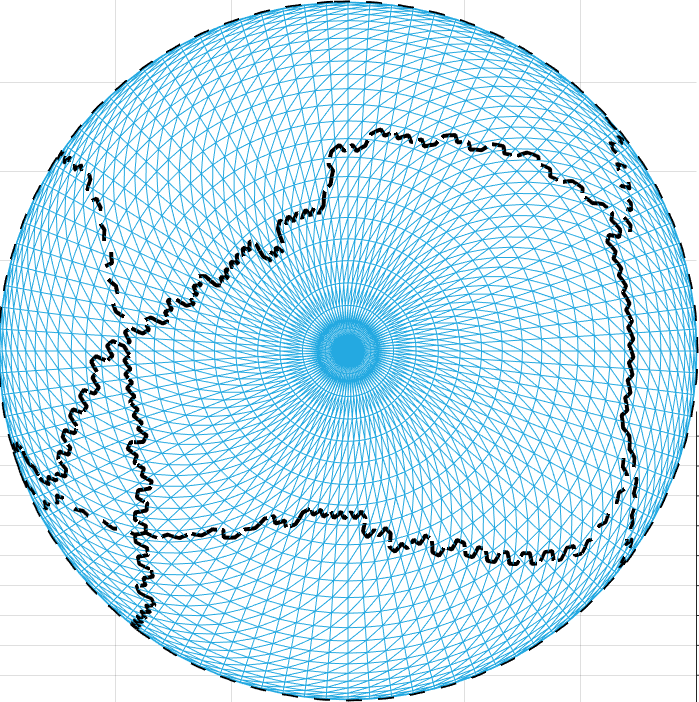
\includegraphics[width = 0.1\textwidth]{figures/TMech_simply_connected_example/design_init_graph}
	\label{fig:TMech_topo_graph}}
\subfigure[]{
	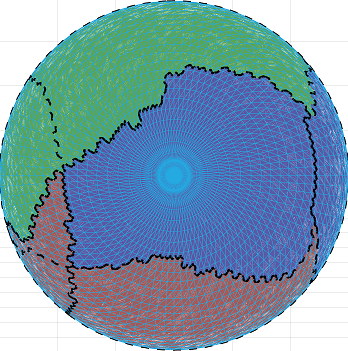
\includegraphics[width = 0.1\textwidth]{figures/TMech_simply_connected_example/design_result_graph}
	\label{fig:TMech_solution}}
\caption{Example of simply-connected cell coverage. (a) Hemispherical object placed in the workspace. 
(b) Simply-connected cells of three valid robot configurations, chosen by the optimal solution shown in (d). 
(c) Topological graph. (d) One optimal solution requiring 2 lift-offs. 
}\label{fig:TMech}
\end{figure}
These cells become the elements on a topological graph Fig.~\ref{fig:TMech_topo_graph}, where each possible colour of a cell is recorded. 
A cellular decomposition splits and merges the cells to transform the process into that of painting all points in the graph with one of the possible colours, driven by attaining a minimum set which equates to a least number of EE lift-offs. 
One such optimal solution with 2 lift-offs is illustrated in Fig.~\ref{fig:TMech_solution}, 
whereby any arbitrary continuous coverage path within a colour surface area will result in maxium joint continuity of the global path. 
\begin{figure*}[t]
\centering
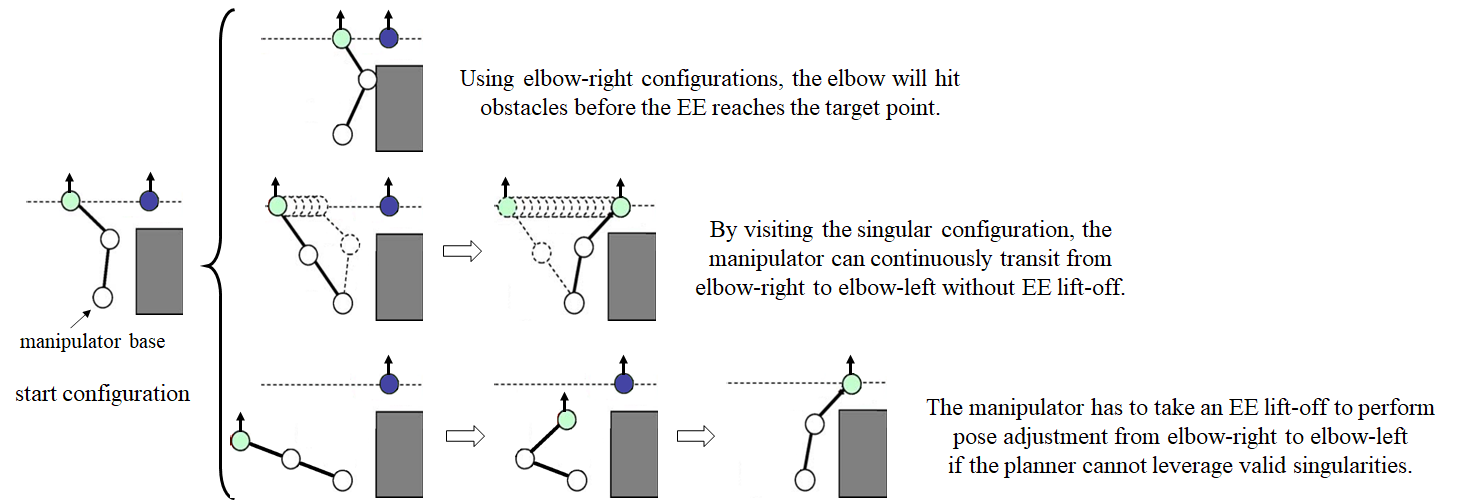
\includegraphics[width = \textwidth]{figures/other_figures/2dof_demo_2}
\caption{
Illustration of using a valid singular configuration to avoid one EE lift-off. To simplify the description the example is taken as a repetitive CPP task. With the last joint keeping the EE perpendicular to the dashed line, the 3DoF RRR manipulator is non-redundant. Starting from an elbow-right pose, the obstacle (gray block) obstructs the smooth EE motion towards the goal pose (the upper case). 
It is apparent that there is a valid singular configuration when the EE moves to the left most, an ``elbow-straight" configuration which smoothly connects the elbow-right poses and elbow-left poses, which reduces the number of lift-off to zero (the middle case). 
If we directly disregard all singular configurations, then one EE lift-off is required (the lower case). 
}\label{fig_2dof_demo}
\end{figure*}
The addition of obstacles and the relative pose of robot and object further condition the final solution. 




\begin{color}{blue}
The kernel assumption of the existing work to NCPP is overlooking the usage of all singularities, which is equivalent to impose a full-rank manipulability constraint to all configurations~\cite{yoshikawa1990translational}. 
As such the forward kinematic mapping from an individual joint-space set to the object surface is ``flat", and arbitrary designing of the geometric coverage paths will induce a continuous joint-space trajectory. 
However, the assumption is too conservative: If the pertubation in some dimensions can be safely disregarded, then only rank-deficient manipulability measures are required, and thus singular configurations may also be valid. 
For example, when the end-effector does not have a twist offset with respect to the last link of the manipulator, there will be no pertubation of EE torque that the manipulator needs to deal with, and one needs not consider the full-rank manipulability measure but the translational manipulability (only the top-$3$ rows of the manipulator Jacobian for a UR5 manipulator)~\cite{yoshikawa1990translational}. 

The valid singularities play crucial roles in performing continuous manipulator motions with the EE restricted on the surface. 
See a planar example in Fig.~\ref{fig_2dof_demo}, where with the EE staying on the dashed line segment (the target ``surface" to be manipulated) and starting with an elbow-right configuration, moving the EE to cover the target point (drawn in purple) becomes a difficult task. 
Keeping elbow-right configurations is not valid as the elbow link will hit the rectangular obstacle (shown in gray). 
However, the transition from elbow-right configurations to elbow-left configurations calls for the usage of a singular ``elbow-straight" configuration. 
Without considering singularities, the algorithm ends up with a solution containing one necessary EE lift-off, whilst by leveraging the singularity to the leftmost reachable point the EE lift-off can be further reduced to zero. 
Further analysing the problem in a realistic scenario gives birth to another problem: 
See Fig.~\ref{fig:discrete_2dof_demo} for illustration. 
When the object is represented by discrete waypoints of EE, there is zero probability to have the singular point captured on the surface. 
As such the path planner is unable to know the joint-space connectedness between elbow-left and elbow-right configurations, and will provide a joint-space path with one EE lift-off to the low-level trajectory generator. 
In particularly, the path will not go leftwards near the singularity, but will carry out an EE lift-off at the beginning and then go rightwards, leaving no possbility for the trajectory optimiser to look for smooth transition visiting the singularity. 

\begin{figure}[t]
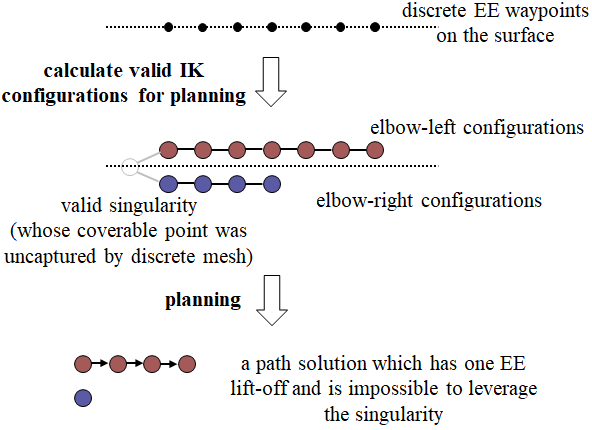
\includegraphics[width=0.48\textwidth]{figures/other_figures/discrete_2dof_demo}
\caption{Illustration of the planning process given discrete waypoints on the task-space. 
Without knowing the valid singular configuration, no connectivity between elbow-left and elbow-right configurations can be observed. }\label{fig:discrete_2dof_demo}
\end{figure}

In summary, following difficulties for solving non-redundant NCPP problem considering smooth transition to valid singularities have been observed: 

\begin{enumerate}
\item Existing model of the non-redundant NCPP problem becomes incomplete when taking valid singular configurations into consideration which may further reduce the EE discontinuities during the coverage task. 
\item Given the non-redundant kinematics of the manipulator, the points on the surface which has valid singular inverse kinematic (IK) solutions are distinct points which cannot be captured by discrete representation of the surface (such as vertices of a mesh). 
Hence valid singularities are not explicit as waypoints for planning. 
%A practical strategy should be proposed to implicitly leverage the singularities for obtaining a minimum number of EE lift-offs. 
\end{enumerate}
And the contributions of this work is summarised as below: 
\begin{enumerate}
\item We provide a complete modelling to the NCPP problem considering singularities. 
We successfully revert the unsolved problem to the solved one considering only non-singular configurations, i.e., a graph with finite number of cells and edges. As such existing graph solvers are applicable to solve the new problem. 
\item By analysing the geometric structure of the joint-space near valid singularities, we show that permissible EE path always exists on analytic surfaces ensuring smooth visiting to the singular point. 
\item We particularly discuss the applicability of the graph solver running on discretely represented surfaces where singularities cannot be explicitly captured. 
A novel mechanism consisting of globally adopting template coverage paths on the target surface and locally adopting path planers for smooth transition to singularities is proposed.  
\end{enumerate}

The remainder of this paper~\footnote{A video illustrating the concepts hereby described can be found 
here:\url{https://youtu.be/TqFzqGGM06Y}} is organised as follows. 
Section~\ref{section_related_works} reviews existing literature. 
Section~\ref{section_problem_modelling} provides definitions and models the singularity-aware NCPP problem into a topological graph with singularity-specified connectivities between colours. 
Section~\ref{section_analytic} considers the lift-off avoidance by visiting the singular configurations, where a permissible direction ensures smooth transition between different sets of non-singular configurations without EE lift-off.
Section~\ref{section_discrete} focuses on the non-existence of valid singular configurations in discretised surface mesh, and presents a practical approach for simultaneously leveraging singularities and adopting template coverage paths. 
Experimental results from simulations and real-world illustrations are collected in Section~\ref{section_exp}, with final concluding remarks gathered in 
Section~\ref{section_conclusion}.
\end{color}

\begin{color}{blue}
\section{Related Works}\label{section_related_works}
The classical solutions of the coverage path planning (CPP) problem consists of two parts: dividing the robot's workspace into simple and easily handled cells, so called the cellular decomposition~\cite{choset2000exact}, and then deforming a template coverage path to fit into each cell. 
The cellular decomposition is directly carried out in the target-space, which for instance is the object surface in the manipulator coverage task. 
Practical approaches are the trapezoidal decomposition~\cite{Seidel1991Simple}, the Morse decomposition~\cite{Acar2002Morse}, Voronoi-based approaches~\cite{Choset2000Sensor-based}, etc. 
When designing the geometric coverage path within each cell, boustrophedon paths~\cite{Choset1998Coverage} and spiral paths~\cite{Hassan2018A} are the most popular solutions. 
Various aspects of coverage performance have been considered~\cite{Atkar2003Towards} for the path generation, such as the time to completion, energy minimisation~\cite{Wu2019Energy}. 
In particularly, various kinematic constraints for coverage can be modelled in the target-space, such as the minimising of the number of turns for mobile robots~\cite{Huang2001Optimal} and reducing the time for pausing of the robot motion to avoid damaging the surface~\cite{Hassan2018A}. 

The non-repetitivity in the classical CPP problem is trivial, as the cellular decomposition is directly carried out on the task-space, leading to all cells non-overlapped. 
\end{color}
However, it is worthwhile noting that despite the apparent similarities in planning with mobile platforms, the discontinuities during the coverage task is inherent to the kinematics of manipulator mechanisms, and as such beyond the scope of bibliograpic works from the mobile robotics community. 
\begin{color}{blue}
If the coverage path is designed without consideration of the manipulator EE reachability, kinematic constraints and environmental factors such as the surrounding obstacles may prevent the manipulator EE from continuous tracking. 
And the coverage path planning became further difficult when revisiting points on the surface is not allowed, referred to as the non-revisiting coverage path planning (NCPP) problem. 
\end{color}
It is arguable that for surface contact tasks in particular, the cost incurred in joint discontinuities significantly 
outweighs other metrics, e.g. by switching between differing geometric paths such as boustrophedon and spirals as proposed in the works~\cite{Hassan2018A}, moreover where undesirable transitions between position and force/torque control~\cite{heck2015switched}~\cite{mirrazavi2018a}~\cite{solanes2018adaptive} become unavoidable.
\begin{color}{blue}
The manipulator NCPP task was firstly modelled as a graph solving problem~\cite{Yang2020Cellular} where the graph consists of purely simply-connected cells, and was then generalised to graph with all cases of multiply-connected cells in~\cite{Yang2020Nonrevisiting}. 
After the graph is solved, within each cell of the graph arbitrary coverage path for the manipulator EE can be adapted, such as the boustrophedon path and the spiral path, with no EE discontinuities during manipulator motion being guaranteed. 
However, these algorithms did not consider the existence of valid singularties which bridge the disconnected configurations but make the forward kinematics non-injective and break the definition of ``colour" in existing solutions (detailed definitions given in Section~\ref{section_problem_modelling}). 
In a contrast, a complete modelling of the non-redundant NCPP problem is proposed in this work. 

\end{color}

\section{Problem Modelling}\label{section_problem_modelling}
\begin{color}{blue}
In this section, we first provide basic definitions for the NCPP problem assuming the non-existence of singular configurations, and prove the finiteness of the number of cells in the topological graph. 
Part of these contents (in Section~\ref{subsection_definitions} and Section~\ref{subsection_regular_finiteness}) have appeared in early work~\cite{Yang2020Nonrevisiting}. 
Then, focusing on the distribution of singularities, we propose a new modelling to the NCPP problem considering singularities. 
\end{color}

\subsection{Definitions and Problem Statement}\label{subsection_definitions}
Define the surface of an object by $M$. 
To simplify the description, let $M$ be only the coverable part of the surface. 
The shape of other obstacles in the workspace and their relative poses in the workcell are assumed static and known.
Given the kinematics of the non-redundant manipulator, we denote the joint-space by $\mathscr{C}$, \textcolor{blue}{which consists of regular (non-singular) configuations $R$ and singular configurations $S$. }
The set of valid non-singular configurations and valid singular configurations are denoted by $\tilde{R}$ and $\tilde{S}$ respectively, where the validity of a configuration is evaluated by some given continuous quality constraints denoted by $\{F_k\}_{k\in \mathbb{N}}$. 
Classic examples of constraints would be manipulability or the minimum distance from an obstacle. 
\textcolor{blue}{Note that $\tilde{R}$ can be explicitly calculated as for each regular EE pose there are only finite number of inverse kinematic solutions for the non-redundant manipulator. In contrast, a point on the surface may admit infinite number of singular IK solutions in $\tilde{S}$. }
The optimal NCPP problem is to find a joint-space path consisting of valid configurations whereby the manipulator EE covers the workspace non-repetitively 
and ensures the least number of discontinuities requiring lifting from the object's surface and least number of EE suspension on the surface deteriorating the performance of the coverage task. 
\textcolor{blue}{
It has been claimed that the thresholds of the given quality constraints can be defined by strict inequalities, i.e., the $k$-th constraint should be expressed as
}
\begin{equation}\label{equ_strict}
F_k(c) > \delta_k = \delta_k(c, F_1, \cdots, \hat{F}_k, \cdots, F_{n}), \forall c\in \mathscr{C}
\end{equation} 
where ``$\hat{\ }$" means excluding the term. $\delta_k$ can be a function of other metrics instead of a constant value, leading to wider applications. 
For example, let $F_1$ represent the manipulability~\cite{yoshikawa1990translational} 
and $F_2$ represent the minimum distance between the manipulator and all obstacles, then an inequality such as
\begin{equation}
F_2(c) > \delta_2 = 0.01+0.05(1-F_1(c))
\end{equation}
could be imposed to indicate that when $F_1(c)$ is small, i.e. the manipulator is in a ``badly-conditioned" configuration, it should be farther from obstacles than would be desirable otherwise. 

\begin{color}{blue}
Without considering singularities, a manipulability constraint is imposed which automatically shapes a gap with joint-space distance threshold $\exists \epsilon_{\rm sing} > 0$,  
\begin{equation}\label{equ_threshold}
d(c, s) > \epsilon_{\rm sing}, \forall c\in \mathscr{C}, \forall s\in S
\end{equation}
where $d(\cdot, \cdot)$ is the joint-space distance metric and $\epsilon_{\rm sing}$ need not be in an explicit form. 
It has been shown that $\tilde{R}$ consists of disjointed sets of non-singular configurations, and within each set the kinematic mapping to the object surface is locally bijective. 
This motivates us to represent each set of configurations by a colour, such as ``blue" or ``red". 
A sub-region of the object surface is said to have possible colour ``blue" if, for any point in the sub-region, one of its IK solutions belongs to the joint-space set assigned with ``blue". 
Then, the distribution of the coverable regions of different colours naturally constructs a topological graph, where the whole surface $M$ is splitted into cells by the reachable boundaries of colours, as per shown in Fig.~\ref{fig:TMech}. 
\end{color}
Precisely, a topological 
cell $C_i$ is defined (where $i$ represents its index) as a maximal set of connected surface points where the valid configurations to cover them are 
pairwise continuous, i.e., $\forall m, m'\in C_i$, let the valid configurations to cover them be 
\begin{equation}\label{equ_pm}
P_{m} = \{c_{m1}, \cdots, c_{mn}\}\subset \tilde{R}
\end{equation}
\begin{equation}\label{equ_pm'}
P_{m'} = \{c_{m'1}, \cdots, c_{m'n'}\}\subset \tilde{R}
\end{equation}
then $n = n'$ and
$\forall c_{mi}\in P_m$, $\exists c_{m'j} \in P_{m'}$ such that $c_{mi}$ and $ c_{m'j}$ are joint-space continuous.
A topological edge $E$ is described by a maximal set of continuous points between $C_i$ and $C_j$
\begin{flalign}
 E & =   \, E(C_i, C_j) \nonumber \\
       & =  \left\{m\in M| \forall (m\in )U_m, \exists m_i, m_j\in U_m, m_i\in C_i, m_j\in C_j\right\}
\end{flalign}
where $U_m$ is an open set containing $m$. 
The topological graph is the ordered cells and edges, $G = (\{C_i\}, \{E_j\})$. 

\begin{color}{blue}
All points in a single cell have the same set of possible colours, and solving the NCPP task is to choose one IK solution from the possible set for each point on the surface, which is visually interpreted as a painting process of the graph. 
Since a connected surface region painted in the same colour admits a continuous manipulator motion without EE lift-off, the NCPP task with minimum EE discontinuities finally translates to the optimal painting problem of the topological graph with least number of colour regions. 

Considering only the non-singular joint-space $\tilde{R}$, a graph solver has been proposed in~\cite{Yang2020Cellular} and~\cite{Yang2020Nonrevisiting}. 
However, for the complete space of valid manipulator configurations $\tilde{R}\cup \tilde{S}$, the manipulator kinematics is no longer flat and admits null motion, which has not been properly modelled. 
\end{color}


\subsection{Finiteness of Cells for Non-Singular Manipulator Configurations}\label{subsection_regular_finiteness}
\textcolor{red}{TODO: Should this subsec be removed? }
%\begin{color}{blue}
%When all singular configurations are disregarded, a manipulability constraint is imposed which automatically shapes a gap with joint-space distance threshold $\exists \epsilon_{\rm sing} > 0$,  
%\begin{equation}\label{equ_threshold}
%d(c, s) > \epsilon_{\rm sing}, \forall c\in \mathscr{C}, \forall s\in S
%\end{equation}
%where $d(\cdot, \cdot)$ is the joint-space distance metric and $\epsilon_{\rm sing}$ need not be in an explicit form. 
%\end{color}
%For a non-redundant manipulator, for any point on the surface $\forall m\in M$, there exist a finite number of valid configurations to cover $m$. 
%By following the constraint laid out in the problem statement, a topological graph will be generated. 
%A sufficient condition to solve it is thus guaranteeing the finitness in the number of cells on this graph. 
%For that, a topological 
%cell $C_i$ is defined (where $i$ represents its index) as a maximal set of connected surface points where the valid configurations to cover them are 
%pairwise continuous, i.e., $\forall m, m'\in C_i$, let the valid configurations to cover them be 
%\begin{equation}\label{equ_pm}
%P_{m} = \{c_{m1}, \cdots, c_{mn}\}\subset \tilde{R}
%\end{equation}
%\begin{equation}\label{equ_pm'}
%P_{m'} = \{c_{m'1}, \cdots, c_{m'n'}\}\subset \tilde{R}
%\end{equation}
%then $n = n'$ and
%$\forall c_{mi}\in P_m$, $\exists c_{m'j} \in P_{m'}$ such that $c_{mi}$ and $ c_{m'j}$ are joint-space continuous.
%A topological edge $E$ is described by a maximal set of continuous points between $C_i$ and $C_j$
%\begin{flalign}
% E & =   \, E(C_i, C_j) \nonumber \\
%       & =  \left\{m\in M| \forall (m\in )U_m, \exists m_i, m_j\in U_m, m_i\in C_i, m_j\in C_j\right\}
%\end{flalign}
%where $U_m$ is an open set containing $m$. 
%Note that the intersecting points of topological edges 
%\begin{equation}
%\{m| \forall (m\in )U_m, \exists m_i, m_j, m_k\in U_m, m_i\in C_i, m_j\in C_j, m_k\in C_k\}
%\end{equation}
%are distinct points, which is negligible when discussing the connectivity of the cells. 
%The topological graph is the ordered cells and edges, $G = (\{C_i\}, \{E_j\})$. 

To prove the finitness of this graph, for each point $m$ with a set of valid 
configurations $P_m$ defined by (\ref{equ_pm}), 
\begin{equation}
F_k(c_{mi}) > \delta_k, \forall k, \forall i = 1, \cdots, N
\end{equation}
the strict inequalities (\ref{equ_strict}) enable us to find valid open sets $U_{mi}$ for each configuration $c_{mi}$ in the joint-space:
\begin{equation}
\begin{aligned}
&\exists (c_{mi}\in )U_{mi} \subset \mathscr{C}, \forall i = 1, \cdots, N \\
\mbox{s.t.}\mbox{  } F_k(c) > \delta_k + &\frac{1}{2}(F_k(c_{mi}) - \delta_k)> \delta_k, \forall k, \forall c\in U_{mi}
\end{aligned}
\end{equation}
since the kinematic function of the manipulator (${\rm FK}$) is continuous and $c_{mi}\in U_{mi}$, 
\begin{equation}
m\in {\rm FK}(U_{mi})\subset M, \forall i = 1, \cdots, N
\end{equation}
so does the intersecting area of those images, 
\begin{equation}\label{equ_finite_intersect}
m\in A_m \triangleq\bigcap\limits_{i = 1}^N\left({\rm FK} (U_{mi})\right)\subset M
\end{equation}
\begin{color}{blue}
The intersection of finite number of open sets is still an open one. 
\end{color}
Following the definition of our topological cells, all points within the intersecting area belong to a same cell. 

For $\forall m\in M$, the corresponding open set $A_m$ exists, as such 
\begin{equation}
\bigcup\limits_{m\in M}A_m\supseteq M
\end{equation}
hence the left term forms an infinite cover of $M$. 
The Heine-Borel Theorem~\cite{Simmons1964Introduction} states that if a compact region can be covered by infinite many open regions, then one can find finite many of them that still fully cover this region. Since all closed sets in the Euclidean space are compact sets, so is the manipulator 
task space in which the boundaries are well-defined. Thus, we can find finite elements from $\{A_m\}_{m\in M}$ that also fully 
cover $M$. Recall that each $A_m$ belongs to only one cell, hence the total number of cells in the graph must be finite. 
\begin{color}{blue}
Thus the sufficiency has been proved.

Inversely, the necessity is easy since the manipulator kinematics is homeomorphic which preserves the closeness and openness of sets. 
Given the cells defined by open sets, the joint-space sets are also open, which means that all constraints that condition the shape of valid joint-space sets need to be described by strict inequalities (i.e., Equ.~(\ref{equ_strict}) and Equ.~(\ref{equ_threshold})).  
%Recall that without the singularities, the manipulator forward kinematic is continuous and injective, and restricted in each continuous set of valid configurations the kinematic is bijective. 
%Since the openness and closeness are invariants under homeomorphic mapping, if we want cells to be boundary-free, the joint-space sets should also be boundary-free, i.e., the joint-space configurations that exactly satisfy the given constraints, staying at the boundary of the set, should be removed. Hence, the validity criteria are described by strict inequalities. 

%In summary, adapting strict inequalities as task constraints is a sufficient and necessary condition for the NCPP problem to be modelled into a well-defined topological graph solving problem. 

\subsection{Modelling of NCPP Considering Singlarities}
\label{subsection_all_finiteness}
When taking valid singular configurations $\tilde{S}$ into consideration, the proof in Section~\ref{subsection_regular_finiteness} is not valid, because there may be an infinite number of valid singular IK solutions ensuring the EE covering the same point on the surface, i.e., (\ref{equ_finite_intersect}) does not hold for finite $N$ at such point. A new modelling to the NCPP considering singularities is presented in this subsection. 

In the new modelling, in order to make the designing of coverage paths easy, we preserve the definition of ``colour", representing a connected joint-space set with pure valid non-singular configurations, as such a connected surface region painted in a single colour still possesses a continuous joint-space manipulator path. 
However, disconnected sets might be connected by valid singularities, graphically the manipulator waypoints (configurations) can transit smoothly from ``red" to ``blue" without EE lift-off. 

We notice that such singular points on the surface must form only zero-area sets. 
The non-redundancy of the manipulator means that given a normal EE pose, the system of kinematics equations is a determinate system. 
When a non-redundant manipulator becomes singular, the system is overdeterminated, i.e., there is zero probability to find a point on the object surface which has infinite many singular IK solutions. 

Let $\{x_{\lambda}\}_{\lambda\in\Lambda}$ be all singular points in a surface $M$, and let $B(x_{\lambda}, \delta_{x_{\lambda}})$ be an open disk on the target surface centering at $x_{\lambda}$ with radius $\delta_{x_{\lambda}}$. 
Then the left-out part of surface
\begin{equation}
\tilde{M} = M\backslash \left\{\bigcup\limits_{\lambda\in\Lambda}B(x_{\lambda}, \delta_{x_{\lambda}})\right\}
\end{equation}
is a surface with closed boundaries and admits only regular surface points which have only non-singular IK solutions. 
By the analysis in Section~\ref{subsection_regular_finiteness}, $\tilde{M}$ has a well-defined topological graph with finite cells for the NCPP problem.  
Let $\delta_{x_{\lambda}}\rightarrow 0^+$, then $\tilde{M}$ converges to $M$ with no area deficiency and whose NCPP problem has been proven finitely solvable. 

Then, we consider adding back the valid singular configurations introduced by the IK solutions of $\{x_{\lambda}\}_{\lambda\in\Lambda}$. 
For the NCPP problem carrying out only in $\tilde{R}$, the number of disjointed joint-space sets is exactly the number of colours, denoted by ${\rm card}\{\tilde{R}\}$. 
Choose a singular point $x_{1}$, denote its singular IK solutions by $\{c_{1\gamma_{1}}\}_{\gamma_{1}\in \Gamma_{1}}\subset \tilde{S}$. 
Since the singular configurations may bridge disjointed sets of non-singular configurations, 
\begin{equation}
{\rm card}\{\tilde{R}\cup \{c_{1\gamma_1}\}\}\leq {\rm card}\{\tilde{R}\}
\end{equation}
Further adding more singularities, we have 
\begin{equation}
\begin{aligned}
&{\rm card}\{\tilde{R}\cup \tilde{S}\}\\
\leq & \cdots\\
\leq&{\rm card}\{\tilde{R}\cup \{c_{1\gamma_1}\}\cup \{c_{2\gamma_2}\}\}\\
\leq&{\rm card}\{\tilde{R}\cup \{c_{1\gamma_1}\}\}\\
\leq&{\rm card}\{\tilde{R}\}
\end{aligned}
\end{equation}
Hence the NCPP problem with valid singularities is modelled into the topological graph constructed on $\tilde{M}$ together with additional colour connectivities introduced by all singularities. 
\end{color}

\begin{color}{blue}
\section{Manipulating with Singularity}\label{section_analytic}
\end{color}
In this section, we focus on analyzing the structure of the joint-space valid configurations near singularities, and prove the existence of a coverage path with joint-space continuity when the object surface is analytic. 
For the rank-deficient manipulability measure, the translational manipulability~\cite{yoshikawa1990translational} is adapted and the Jacobian has one column co-rank at the singular configuration. 
%Recall that we refer the points on the surface that can be covered by singular configurations as singular points, thus all ``points" are in the task-space and all ``configurations" are in the joint-space. 
The main result of this section is: \textbf{Compared with disregarding all singularities, by properly designing the instant motion direction when the EE visits the singular point, the manipulator can perform a smooth transition between configurations belonging to different colours, further avoiding EE lift-offs. }

\subsection{Dimension Analysis and Choice of Frame}
Let the velocity relation between the EE and the joint-angles be as follows: 
\begin{equation}\label{equ_total}
\left[
\begin{matrix}
v_x\\
v_y\\
v_z\\
\omega_x\\
\omega_y\\
\omega_z
\end{matrix}
\right]= \left[
\begin{matrix}
\bar{J}_{5\times 5}\\
\bar{N}_{1\times 5}
\end{matrix}
\right]\left[
\begin{matrix}
\omega_1\\
\omega_2\\
\omega_3\\
\omega_4\\
\omega_5
\end{matrix}
\right] + \left[
\begin{matrix}
0\\
0\\
0\\
0\\
1
\end{matrix}
\right]
\omega_{ee}
\end{equation}
where the left term is the $SE(3)$ tranlational and rotational velocity of an orthonormal frame defined at the contact point between the EE and the surface, $\omega_i, i = 1, \cdots, 5$ are the joint velocities, and $\omega_{ee}$ is the rotational speed of the EE. Here we explicitly write the equation in $6$ dimensions because $\omega_z$ has a physical meaning, the rotational velocity about $z$-axis of the EE, which we can safely ignore given the rotating nature of the EE. Then the reduced joint space motion is 
\begin{equation}
\dot{\bar{x}}_{5\times 1} = \bar{J}_{5\times 5}\bar{\omega}_{5\times 1}
\end{equation}
where $\dot{\bar{x}} = \left[ v_x, v_y, v_z, \omega_x, \omega_y \right]^T$, $\bar{\omega} = \left[ \omega_1, \omega_2, \omega_3, \omega_4, \omega_5 \right]^T$.

\textbf{Dimension Analysis. }
The results mainly come from previous work~\cite{Singh1993Motion}, where the most significant points are the definition of the \textit{accessible space} and the \textit{modified joint-space}. Here we briefly re-state it and show its direct application on the coverage task of 5DoF non-redundant manipulator. 

To diagonalize the matrix, we apply the \textit{singular value decomposition}~\cite{} to $\bar{J}$, 
\begin{equation}
\bar{J} = \bar{U}\bar{\Sigma}\bar{V}^T
\end{equation}
where $U, V$ are orthonormal matrices, and $\bar{\Sigma}$ is not of full rank since the manipulator is singular, 
\begin{equation}
\bar{\Sigma} \triangleq \left[
\begin{matrix}
\sigma_1 &&&&\\
& \sigma_2 &&&\\
&& \sigma_3 &&\\
&&& \sigma_4 &\\
&&&& 0
\end{matrix}
\right],\ \sigma_1 > \sigma_2 > \sigma_3 > \sigma_4 > 0
\end{equation}
The \textit{accessible space coordinates} of $\dot{\bar{x}}$ is defined as 
\begin{equation}
\dot{\hat{x}} = \bar{U}^T \dot{\bar{x}}
\end{equation}
and the \textit{modified joint-space velocity} is defined as 
\begin{equation}
\hat{\omega} = V^T\bar{\omega}
\end{equation}
so the work space motion can be resolved only if expressed in the modified joint space its last component vanishes, which is call the motion on the \textit{restricted sub-manifold}
\begin{equation}
S_x = \{\dot{\hat{x}}_5 = 0\}
\end{equation}
This can be further clarified after we decompose the whole joint-space motion into two orthogonal components, 
\begin{equation}
\bar{\omega}^- \triangleq \bar{V}\hat{\omega}^- = \bar{V}\left[
\begin{matrix}
\hat{\omega}_1\\
\hat{\omega}_2\\
\hat{\omega}_3\\
\hat{\omega}_4\\
0
\end{matrix}
\right],\ \bar{\omega}^\perp \triangleq \bar{V}\hat{\omega}^\perp = \bar{V}\left[
\begin{matrix}
0\\
0\\
0\\
0\\
\hat{\omega}_5
\end{matrix}
\right]
\end{equation}
where $\bar{\omega}^-$ leads to an actual $4$-dimensional motion of the EE in the 5DoF task-space, and $\bar{\omega}^\perp$ only performs the \textit{null motion}.

\textbf{Choice of Local Frame. }
Following the above definitions, we define a local orthonormal frame $\{x; e_1, e_2, e_3\}$ at the contact point as 
\begin{equation}
\left\{
\begin{aligned}
&e_3\mbox{: The unit outer normal vector of $M$ at $x$}\\ 
&e_1\mbox{: The axis that the EE can rotate about}\\ 
&e_2 = e_3\times e_1
\end{aligned}
\right.
\end{equation}
By the definition of $\omega^-$ and $\omega^\perp$ we know that $e_1$ is the rotation axis of $\omega^-$, and the EE cannot rotate about the $e_2$ axis. 

\subsection{Parameterization of Permissible Path}\label{subsection_parameterization}
When the manipulator visits a singular configuration, the EE is no longer locally omni-directional in the task space, but loses the ability of moving in the \textit{degenerate direction}~\cite{Egeland1991Manipulator} which is rotating about the $e_2$ axis based on our definition of local coordinates. 
Since the EE motion is essentially a constrained motion in the surface curvilinear coordinate, i.e., a 2D motion, losing the capability of moving in one dimension means it can only move in the other dimension. 
Hence, at the singular point the \textit{permissible path} is a joint-space smooth path with specified tangent.
In this case, the EE can smoothly traverse the singular point without lift-off. 

We use the Gauss mapping for better visualization. 
The Gauss mapping is a translational movement of the outer unit normal vector from the point on the surface to the origin, which describes the curvature of the surface,
\begin{equation}
g: M\rightarrow \mathbb{S}^2,\ x\mapsto g(x)
\end{equation}
It induces a tangent mapping from the tangent plane $T_xM$ to the tangent space of $\mathbb{S}^2$ at $g(x)$,
\begin{equation}
\begin{aligned}
g_*: T_xM&\rightarrow T_{g(x)}\mathbb{S}^2\\
u&\mapsto g_*u
\end{aligned}
\end{equation}
where $u$ is any tangent vector of $M$. 

\begin{figure}[t]
\centering
\subfigure[]{
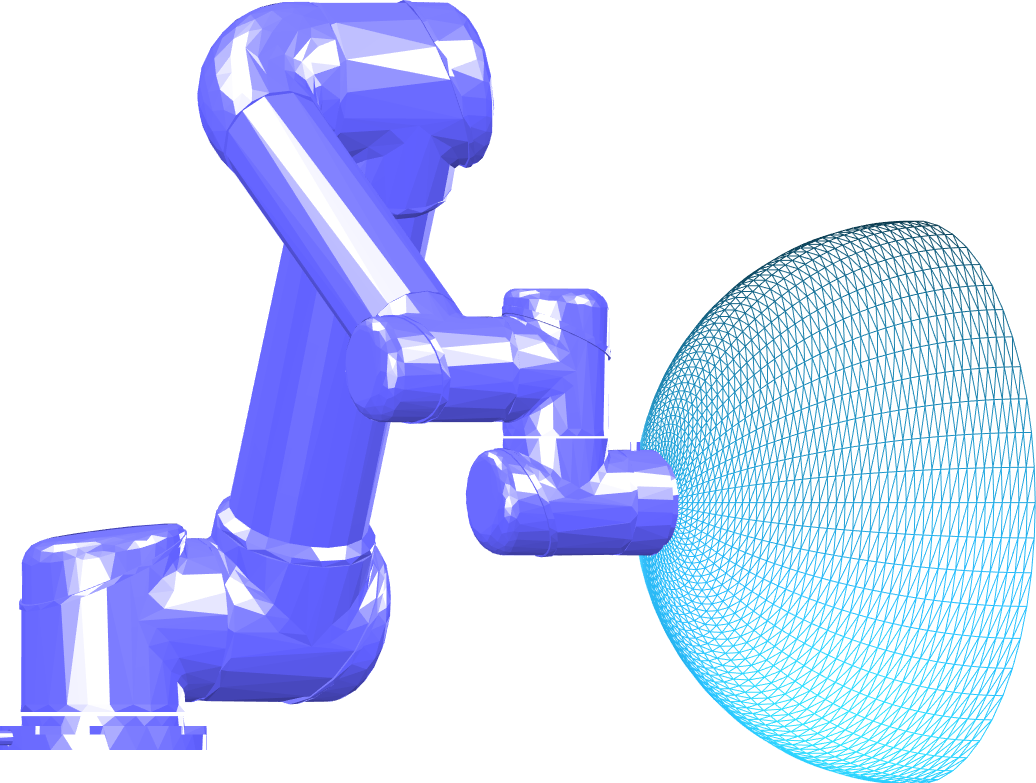
\includegraphics[width = 0.14\textwidth]{figures/other_figures/hemi_demo/center_90}\label{fig:isolated:a}
}
\subfigure[]{
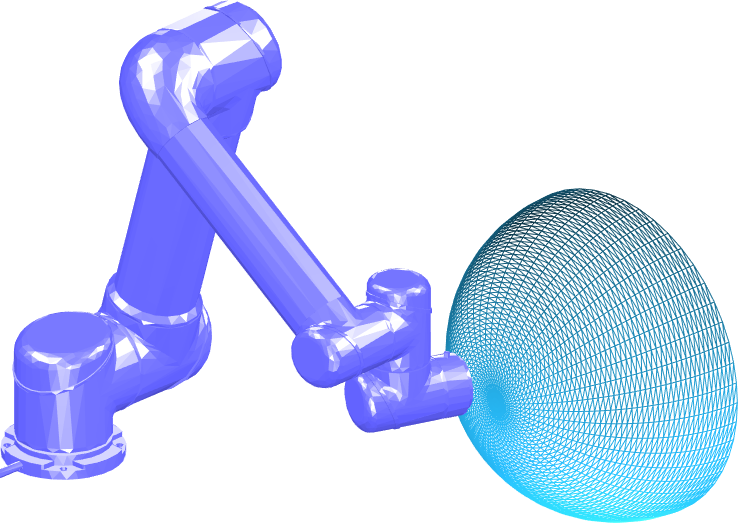
\includegraphics[width = 0.14\textwidth]{figures/other_figures/hemi_demo/offset_90_1}\label{fig:isolated:b}
}
\subfigure[]{
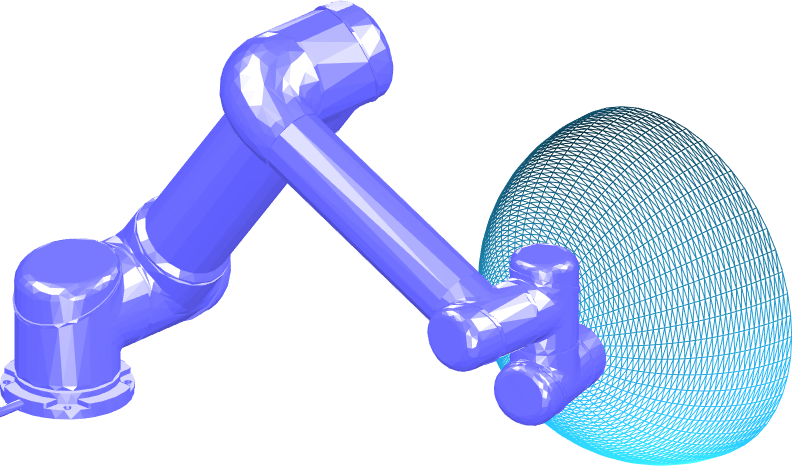
\includegraphics[width = 0.14\textwidth]{figures/other_figures/hemi_demo/offset_90_2}\label{fig:isolated:c}
}
\subfigure[]{
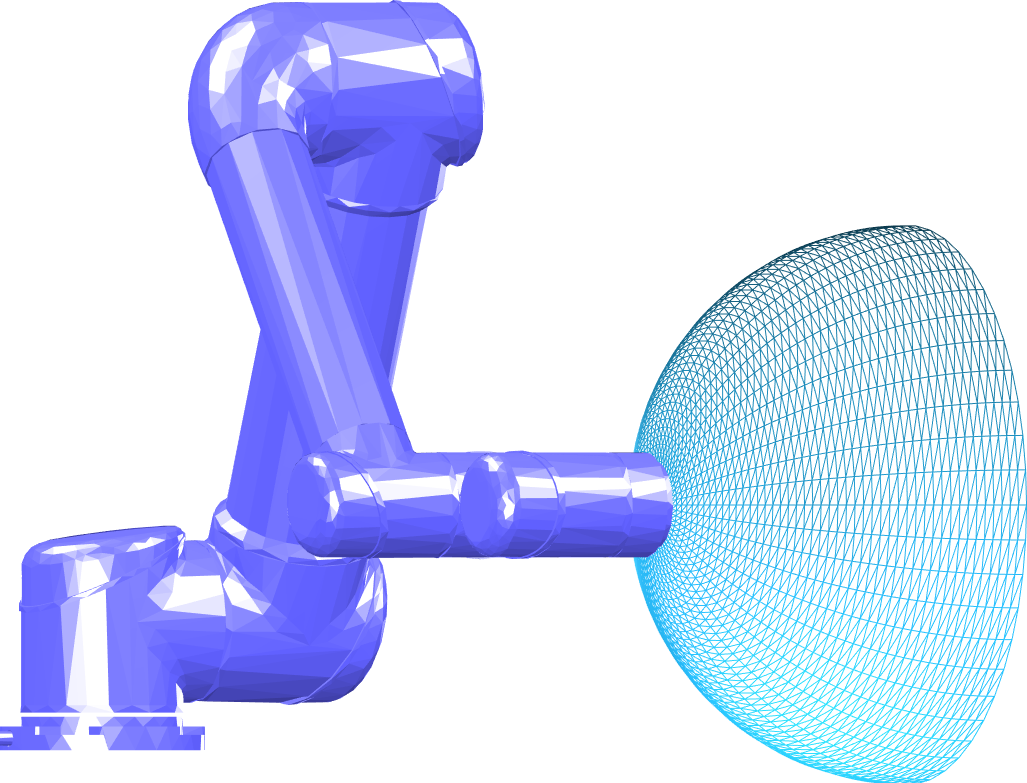
\includegraphics[width = 0.14\textwidth]{figures/other_figures/hemi_demo/center_180}\label{fig:isolated:d}
}
\subfigure[]{
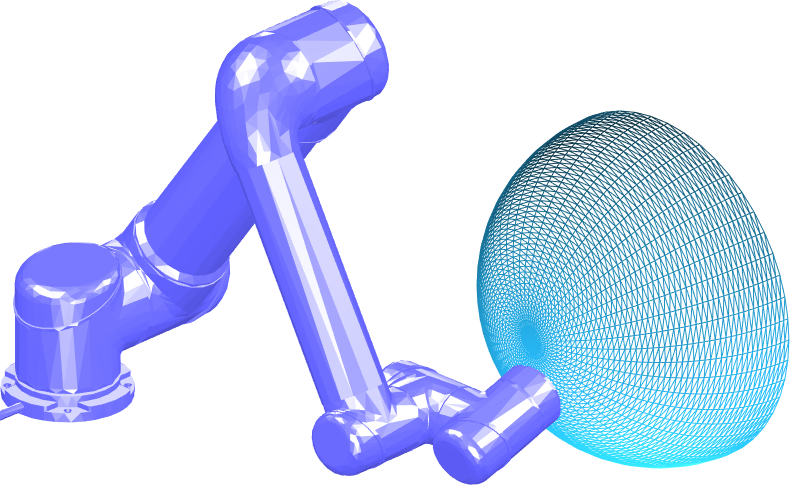
\includegraphics[width = 0.14\textwidth]{figures/other_figures/hemi_demo/offset_180_1}\label{fig:isolated:e}
}
\subfigure[]{
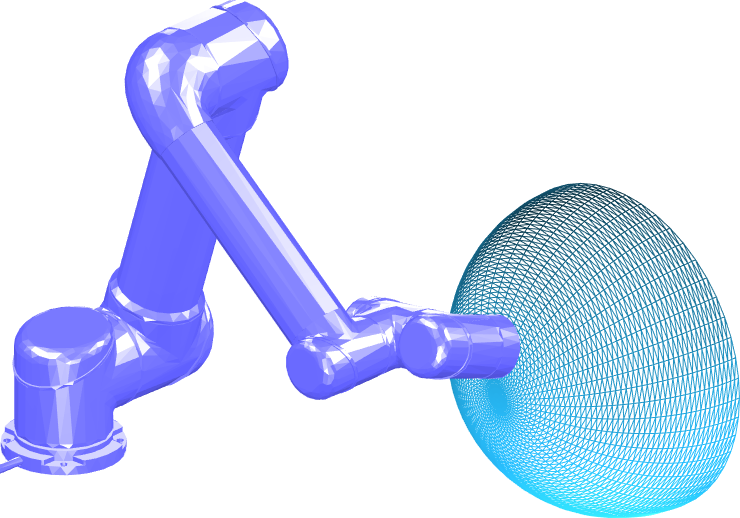
\includegraphics[width = 0.14\textwidth]{figures/other_figures/hemi_demo/offset_180_2}\label{fig:isolated:f}
}
\caption{Illustration of a coverage task with isolated singular point. (a)(d) Valid singular configurations. (b)(c) The non-singular configurations which can be smoothly reached from (a). (e)(f) The non-singular configurations which can be smoothly reached from (d). 
}\label{fig:isolated}
\end{figure}


\begin{figure}[t]
\centering
\subfigure[]{
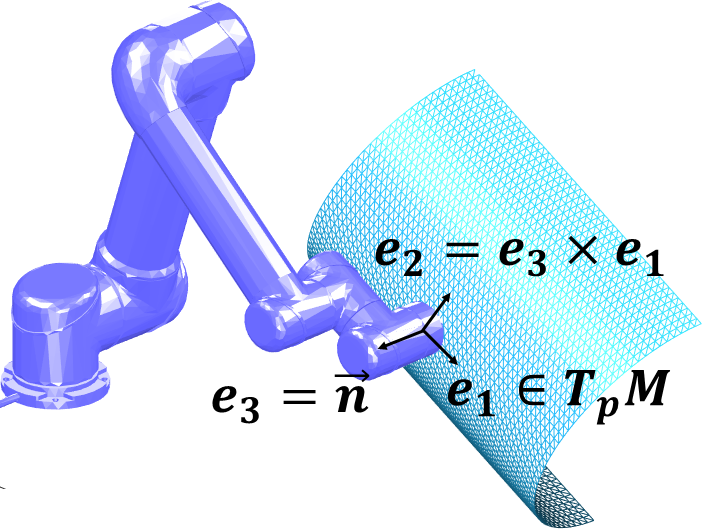
\includegraphics[width = 0.14\textwidth]{figures/other_figures/cylinder_demo/parallel_with_frame}\label{fig:curved:a}
}
\subfigure[]{
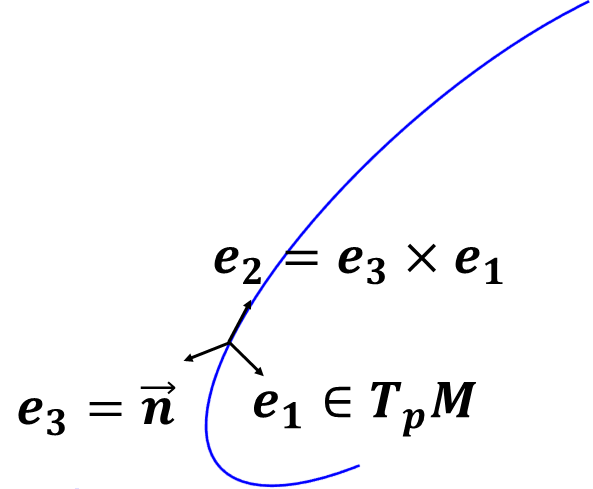
\includegraphics[width = 0.14\textwidth]{figures/other_figures/cylinder_demo/gauss_image_parallel}\label{fig:curved:b}
}
\subfigure[]{
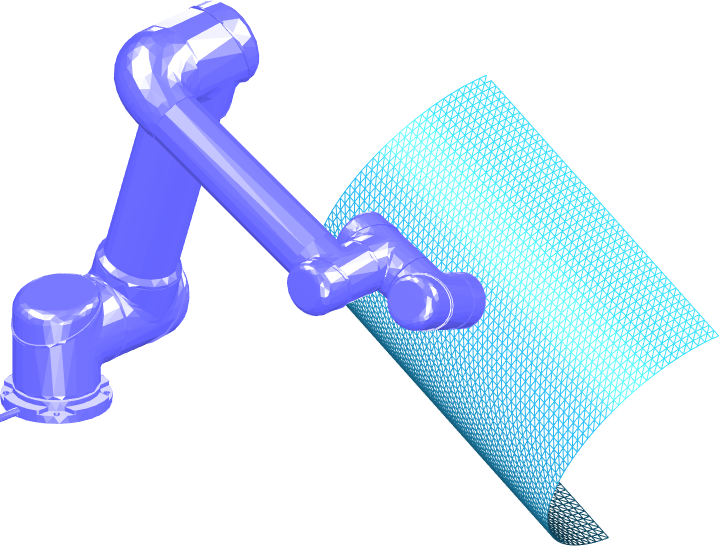
\includegraphics[width = 0.14\textwidth]{figures/other_figures/cylinder_demo/offset_parallel}\label{fig:curved:c}
}
\subfigure[]{
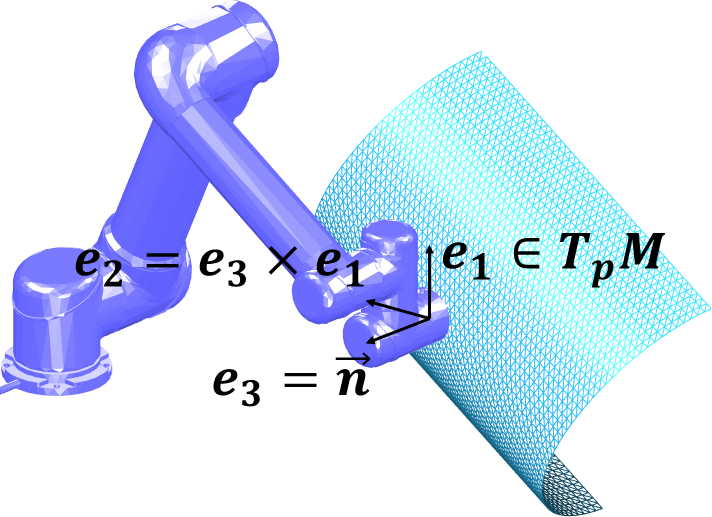
\includegraphics[width = 0.14\textwidth]{figures/other_figures/cylinder_demo/center_90_with_frame}\label{fig:curved:d}
}
\subfigure[]{
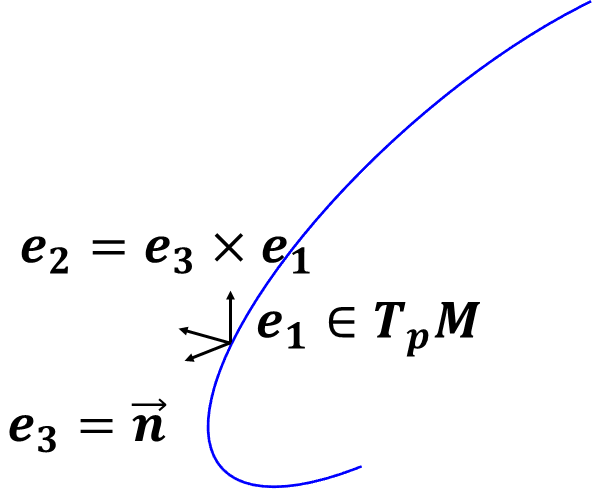
\includegraphics[width = 0.14\textwidth]{figures/other_figures/cylinder_demo/gauss_image_perp}\label{fig:curved:e}
}
\subfigure[]{
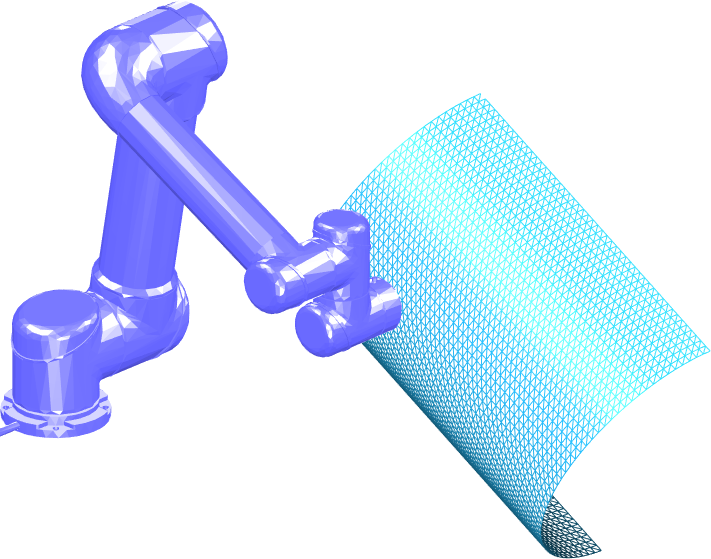
\includegraphics[width = 0.14\textwidth]{figures/other_figures/cylinder_demo/offset_90}\label{fig:curved:f}
}
\caption{Illustration of a curve of singular points where the Gauss mapping is not bijective. (a) A valid singular configuration which can both moving along the permissible direction and moving along the generatrix by EE pure translational motion. (b) The Gauss mapping of (a). (c) The non-singular configuration which can be smoothly reached from (a). 
(d) A valid singular configuration whose permissible direction is not aligned with the surface normal. (e) The Gauss mapping of (d). (f) Another valid singularity which can be visited from (d). 
}\label{fig:curved}
\end{figure}

In the first case, let the Gauss mapping around $x$ be bijective.
For any path $\gamma$ on the sphere passing $g(x)$, 
\begin{equation}\label{equ_gamma}
\forall \gamma: [-1, 1]\rightarrow \mathbb{S}^2, 0\mapsto g(x)
\end{equation}
satisfying that its tangent at $g(x)$ is restricted to 
\begin{equation}\label{equ_gamma_direction}
\frac{d\gamma(s)}{ds}|_{s = 0} // g_*(e_2)
\end{equation}
we can always find its preimage, a path $\gamma_M$ on the surface, satisfying that 
\begin{equation}\label{equ_gammam}
g(\gamma_M) = \gamma\Rightarrow \gamma_M = g^{-1}(\gamma)
\end{equation} 
Then $\gamma_M$ is a permissible path that is smoothly traversable because $g_*$ is a homogeneous tranformation, 
\begin{equation}\label{equ_gamma_para}
\frac{d(g^{-1}(\gamma(t)))}{ds}|_{t = 0} // e_2
\end{equation}
which means that the instant motion of the EE tracking $g^{-1}\comp\gamma$ need not rotate about $e_2$. 
So the coverage path can smoothly visit the singularity as long as we precisely design the tangent of the coverage path to satisfy (\ref{equ_gamma_para}). 

For example, in Fig. \ref{fig:isolated} there is a singular point in the center of a wok-like object, because when the EE is covering the central point, the $2$-nd, $3$-rd and $4$-th joints of the manipulator are rotating in a same 2D plane, as shown in Fig. \ref{fig:isolated:a} and Fig. \ref{fig:isolated:d}. However, it is easy to verify that they are still valid in the sense of translational manipulability. 
The surface is part of a sphere, so the Gauss mapping is equivalent to shrinking the surface to the unit sphere and is omitted in the figure. 
The configurations shown in Fig.~\ref{fig:isolated:b} and Fig.~\ref{fig:isolated:c} are the continuous configurations that are smoothly traversable from the one shown in Fig.~\ref{fig:isolated:a}, from which the EE can only move horizontally. 
And Fig.~\ref{fig:isolated:e} and Fig.~\ref{fig:isolated:f} are continuous to Fig.~\ref{fig:isolated:d}, from which the EE can only move vertically. 

In the second case, the Gauss mapping may not be bijective. 
The preimages of a same point under Gauss mapping can be a connected set of points which have parallel unit outer normal vectors, the EE motion among whom does not require any rotation. 
As such a joint-space motion with pure translational motion is allowed when the manipulator is singular. 
%Hence, if the surface has a locally planar region (curve) around $x$ that allows pure translational motion, besides $\gamma_M$ constructed as above, the EE may alternatively choose any coverage path within the planar region. 

For such an example see Fig.~\ref{fig:curved}. 
The object is part of a cylinder, whose unit normal vectors are parallel along the generatrix, so the Gauss image is only an arc in the unit sphere. 
When the manipulator is at a singular configuration like shown in Fig.~\ref{fig:curved:a}, the $g_*(e_2)$ axis is tangent to the Gauss image of the cylinder, so the manipulator is able to perform motion in two dimensions, along the generatrix (through pure translational motion of EE) and perpendicular to the generatrix (shown in Fig.~\ref{fig:curved:c}). 
%The case remains the same if the wrist joint flips exactly $\pi$ rad. 
However, for other valid singular configurations such as the one shown in Fig.~\ref{fig:curved:d}, except the tranlational motion along generatrix, the manipulator cannot track any path with nontrivial Gauss image on the semicircle, because all of them have non-zero projection on the $g_*(e_1)$ axis, thus require rotational motion about the $g_*(e_2)$ axis. 
To establish EE path tracking, it has to firstly perform a null motion for pose estimation to another singular configuration as shown in Fig.~\ref{fig:curved:a}. 
%However, note that the manipulator can simultaneously perform translational motion along the generatrix as shown in Fig.~\ref{fig:curved:f}, so the EE need not to suspend on the object surface as long as the coverage path takes special consideration. 

\begin{figure}[t]
\centering
\subfigure[Configurations represented by arrows]{
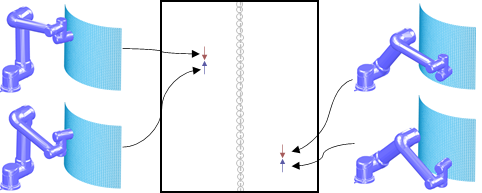
\includegraphics[width=0.48\textwidth]{figures/other_figures/arrow_example_a}
}
\subfigure[]{
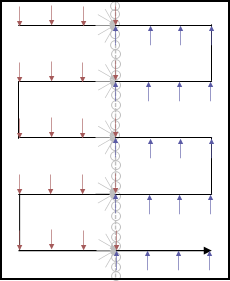
\includegraphics[width=0.22\textwidth]{figures/other_figures/arrow_example_b}
}
\subfigure[]{
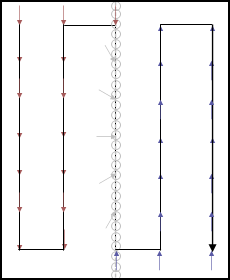
\includegraphics[width=0.22\textwidth]{figures/other_figures/arrow_example_c}
}
\caption{Examples of different coverage paths that has/does not have EE suspensions on the object surface. 
(a) Demo configurations represented by arrows. 
(b) A coverage path in which null motions need to be inserted during path tracking. 
(c) A coverage path which allows the manipulator adjust its poses during EE translational motion, hence no EE suspension is required. }\label{fig:paths}
\end{figure}

One remark for the generation of coverage paths that visit singularities is that, there always exists a smooth manipulator motion visiting the singularities which contains neither EE lift-offs nor EE suspension on the object surface.  
\begin{color}{blue}
See different coverage paths designed on the cylinder example in Fig.~\ref{fig:paths}. 
The cylinderical surface is mapped to a planar region for easy illustration of the coverage paths. 
Two kinds of configurations are distinguished which differ at the wrist-joint (upwards or downwards), represented by arrows pointing at different directions. 
Gray circles mark the position of singular points on the surface, and gray arrows represent the valid singular configurations which were not selected as manipulator waypoints. 
If the coverage path goes across the curve of singular points, then the manipulator has to adopt a null motion with the EE pausing on the singular point, marked by multiple gray arrows pointing at the same point. 
In contrast, if the coverage path has an aligned part with the singular points, then the manipulator can adjust its pose during the translational motion of the EE on the surface. 

%In summary, no matter how many degrees of freedom that the non-redundant manipulator has, since the EE motion on the surface of the object is a 2D one, if the manipulator is in a valid singular configuration under rank-deficient manipulability constraints, losing the capability of the EE moving in one dimension means there is only one dimension left, leading to a restricted motion direction of the coverage path on the singular point. Thus through properly design the motion direction of the EE when passing the singular points, the manipulator can smoothly track the coverage path without EE lift-off or suspension. 


\begin{figure*}[t]
\centering
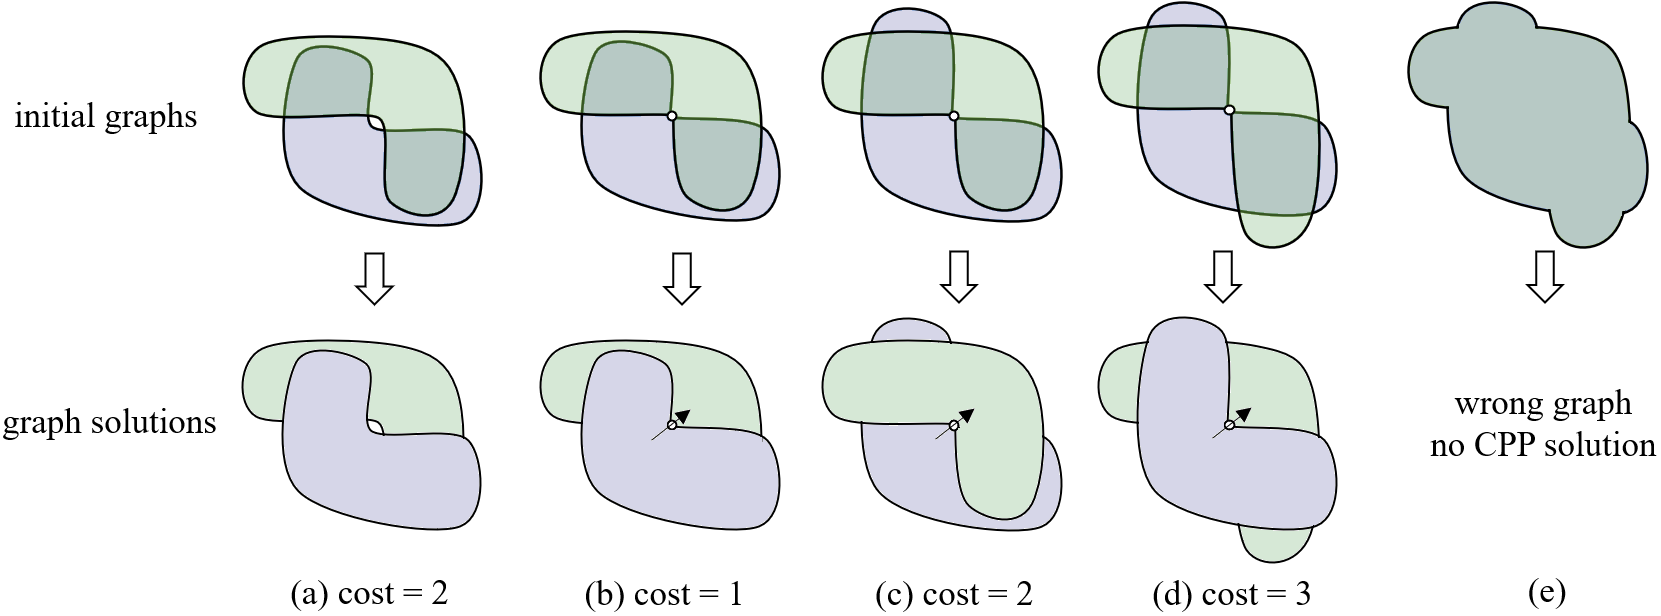
\includegraphics[width=0.96\textwidth]{figures/other_figures/cost}
\caption{Illustration of different graphs and one of their optimal solutions. 
The cost is the number of continuous manipulator motions for the NCPP task. 
(a) Without using the singular configurations, the central point is uncoverable, and the coverage task requires one EE lift-off. 
(b) If the manipulator transits from blue to green by visiting the singularity during which the EE visits the central round point, a continuous coverage path without EE lift-off can be constructed. 
(c)(d) The connectivity between colours is only local, so EE lift-offs are still required if the colours have mutual interruptions. 
(e) Combining the blue colour and the green colour and assigning all their corresponding configurations the same colour will give a wrong topological graph. 
}\label{fig:cost}
\end{figure*}

\subsection{Graph Solver Containing Singularities}
When solving the topological graph using existing graph solvers, for each step during the solving process, the graph is partly painted, and the physical meaning of the current ``cost" is the number of painted regions in the partly solved graph. 
The cost variations caused by each singularity needs extra consideration: 
\begin{equation}
\Delta cost_{x_\lambda} = 1 - j
\end{equation}
where $j$ is the connectable painted regions of point $x_\lambda$ which were disconnected before envolving the singular IK solutions of $x_\lambda$. 
When designing the geometric coverage paths after the graph is solved, different parts of the continuous ``colour-crossing" coverage paths are firstly designed in each cell and then concatenated by the singularties. 

It is noticeable that the connectedness of different colours introduced by valid singularities is local. See the difference between examples shown in Fig.~\ref{fig:cost}. 
Although the blue colour and the green colour can be smoothly connected by visiting the singularities, it does not mean the overlapping of their coverable areas can always be manipulated without EE lift-off. 
It will cause wrong calculation of costs if different colours bridged by singularities are directly merged into a single one in the initial topological graph. 
Unfortunately, this is inevitable when the surface is not analytic but discretely represented, which is to be discussed in the next section. 
\end{color}


\section{SNCPP in Discretized Data}\label{section_discrete}
Now we assume the object surface is discretely represented by a mesh. 
Since the points on the surface corresponding to singular IK solutions only form zero-area region, finitely sampling some waypoints has zero probability to know the exact position of the singular points. 
What makes the problem further complicated is that we can neither explicitly leverage the null space path during coverage planning, because a null space path only corresponds to a single EE point on the object surface. 

It is observed that two consecutive waypoints indicate a straight path segment connecting them, so even if a singular point is not in the waypoints of the coverage path, the coverage path may still visit it as long as two waypoints stay opposite to it. 
In this section, we present the necessary and sufficient condition to leveraging singularities without precise knowledge about their positions, and propose a practical approach to both leveraging the singularities and adopting template CPP solutions. 

\begin{figure}[t]
\centering
\subfigure[]{
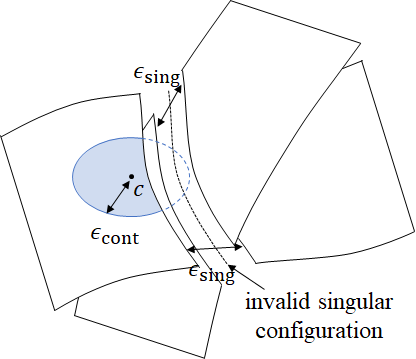
\includegraphics[width=0.22\textwidth]{figures/other_figures/cspace_gap}\label{fig:gap:a}
}
\subfigure[]{
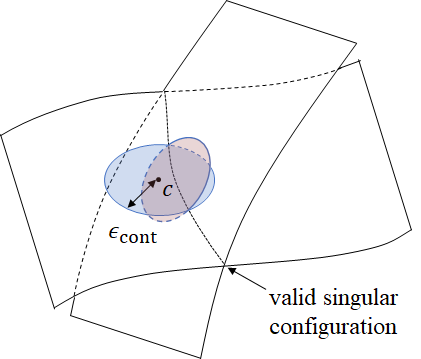
\includegraphics[width=0.22\textwidth]{figures/other_figures/cspace_nogap}\label{fig:gap:b}
}
\caption{Structure of valid configurations near singularities. If the singular configuration cannot satisfy the manipulability constraint, then a gap exists between the singular configurations and the valid configurations with width $\epsilon_{\rm sing}$. For $\epsilon_{\rm cont} < \epsilon_{\rm sing}$, regarding $\epsilon_{\rm cont}$ as a threshold of judging the continuity of configurations, the algorithm always performs correctly. However, for the valid singular configurations, there does not exist such a gap, thus for any precision of $\epsilon_{\rm cont}$, the algorithm will inevitably make mistakes.
}\label{fig:gap}
\end{figure}


\subsection{Distance-based Continuity Measure}
For discrete joint-space configurations, the algorithm has to use a discrete distance threshold for judging the continuous configurations, such as
\begin{equation}\label{equ_continuous}
\forall c_1, c_2\in \mathscr{C}, c_1, c_2\mbox{ are continuous}\Leftrightarrow d(c_1, c_2) < \epsilon_{\rm cont}
\end{equation}
where $d(\cdot, \cdot)$ is the joint-space distance, and $\epsilon_{\rm cont} > 0$ is a pre-determined joint-space distance threshold. 
$\epsilon_{\rm cont}$ depends on the resolution of the mesh and $\epsilon_{\rm sing}$. 
When the mesh is of higher quality, the configurations covering adjacent vertices on the mesh have a smaller joint-space difference, which is good for judging joint-space continuity. 
However, for sparse mesh, $\epsilon_{\rm cont}$ has to be a little bigger so that two discrete but essentially continuous (without passing singularity) configurations can be still correctly regarded as continuous. 
And $\epsilon_{\rm cont}$ should be less than $\epsilon_{\rm sing}$ so that the algorithm would not mistakenly see two configurations (passing invalid configurations) as continuous. See Fig.~\ref{fig:gap:a} for illustration. Note that $\epsilon_{\rm sing}$ is in an implicit form, so $\epsilon_{\rm cont}$ is chosen as small as possible to avoid violation. 
(This also indicates that the mesh cannot be too sparse, or else no suitable $\epsilon_{cont}$ can be found: either some continuous configurations are assigned with different colours, or some discontinuous configurations are assigned the same colour.)
However, it is noticable that when there exist valid singularities, no matter how small $\epsilon_{\rm cont}$ is, the distance-based connectivity measure will always make wrong judgement, because the valid singularities amidst two non-singular sets have zero-area, i.e., $\epsilon_{\rm sing} = 0$. 
See Fig.~\ref{fig:gap:b} for illustration. 
\begin{color}{blue}
%Implicitly labelling configurations which are only connectable by visiting singularities as a same colour will break the construction of the topological graph, concretely, make the kinematic mapping from the coverable area of a colour to its joint-space configurations non-bijective, causing the problem shown in Fig.~\ref{}. 


\subsection{Adoption of Null Motion}
The existence of null motion is intuitive following the illustration in Fig.~\ref{fig:indicated}, where the joint-space path that connects two waypoints (configurations) is off the constrained manifolds. 
In other words, the coverage path constructed on object surface did not provide a trackable joint-space trajectory for the subsequent low-level controller. 
In the controlling stage, a controller might have a more precise model than the coverage planner about the local structure of the joint-space, maybe an analytic model of the surface, and thus may be able to modify the untrackable path onto the constrained manifolds and generate valid joint-space trajectories, within which the singularities appear. 
(Or else the trajectory controller will report a failure in creating a feasible joint-space trajectory and introduce an EE lift-off for path tracking.)
However, note that the modification of trajectory given by controller will cause an unexpected motion of the EE on the object surface. 
The coverage path, i.e. the trace of EE, cannot be arbitrarily adjusted for ensuring full coverage and non-repetitivity (an example will be given in Fig.~\ref{fig:bad_mesh}). 
This calls for a mechanism to find consecutive waypoints that are aligned with the permissible direction of the singularity. 
As such the modified joint-space trajectory will not have null motion and the EE will precisely track the predefined coverage path. 
See Fig.~\ref{fig:better} for a better coverage path indicated by discrete waypoints. 
\end{color}

\begin{figure}[t]
\centering
\subfigure[]{
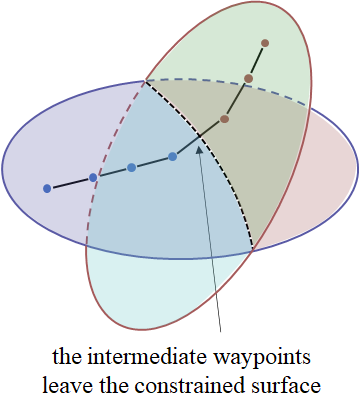
\includegraphics[width=0.22\textwidth]{figures/other_figures/demo_planning_path}
}
\subfigure[]{
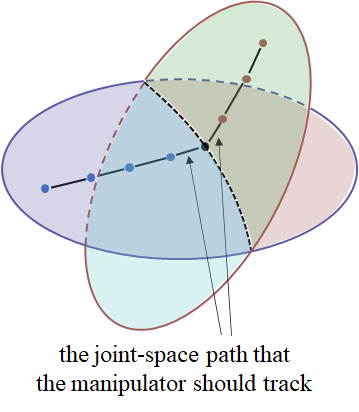
\includegraphics[width=0.22\textwidth]{figures/other_figures/demo_controlling_path}\label{fig:indicated:b}
}
\caption{Without the singular configuration as a waypoint, the indicated joint space motion given by the CPP planner is not trackable. If the tracking problem is solved by carrying out trajectory modification by the low-level controller, then the EE will have unexpected movement on the object surface and will pause on the surface during the manipulator null motion. 
}\label{fig:indicated}
\end{figure}

\begin{figure}[t]
\centering
\subfigure[]{
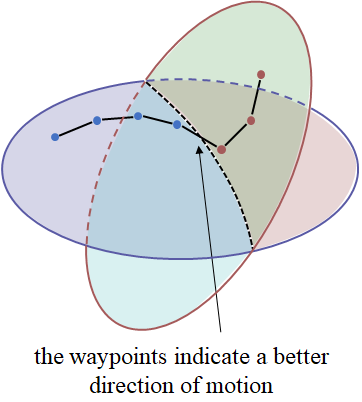
\includegraphics[width=0.22\textwidth]{figures/other_figures/demo_better_planning_path}
}
\subfigure[]{
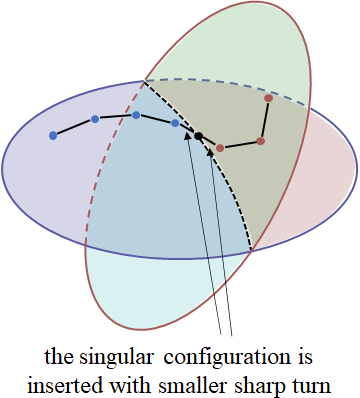
\includegraphics[width=0.22\textwidth]{figures/other_figures/demo_better_controlling_path}
}
\caption{Illustration of a better solution of the case in Fig.~\ref{fig:indicated}. Although the waypoints neither contain a singular configuration, the motion orientation of the two waypoints makes the indicated straight path closer to the singularity. 
Then after the path be optimized to a continuous trajectory by a low-level controller, it contains a smaller sharp turn. Ideally, there exists one motion direction (the permissible path) that the straight path implicitly passes the singular point, and there will be no sharp turn in the optimized joint-space trajectory. 
}\label{fig:better}
\end{figure}

\subsection{Condition for Asymptotically Smooth EE Motion}\label{subsection_asymptotical}
We claim that the necessary and sufficient condition of leveraging singular points on discretized data structure is that, the sampling strategy of waypoints is asymptotically finding all elements in the unit tangent bundle of the surface. Here the unit tangent bundle is the set of all unit tangent vectors of all points on the surface $M$, denoted by $UM$, which is a 3D space. 

The sufficiency is intuitive to show if each waypoint indicates an instant motion direction when the EE visits it. 
As the waypoints are incrementally sampled, we can find a waypoint which is arbirarily close to the desired ``singular point position -- permissible direction" pair. 

The necessity is also easy by constructing a counterexample. If there exists a point on the surface whose unit tangent space is not asymptotically completely sampled, then we may precisely choose a special pose of the object to put this point to EE position of a singular configuration with the permissible orientation be just overlooked by the incomplete sampling process. Unable to find a smooth joint-space path visiting the singular point, the result joint-space path has to either perform one EE lift-off, or perform an unexpected EE motion caused by joint-space trajectory modification.

\begin{figure}[t]
\centering
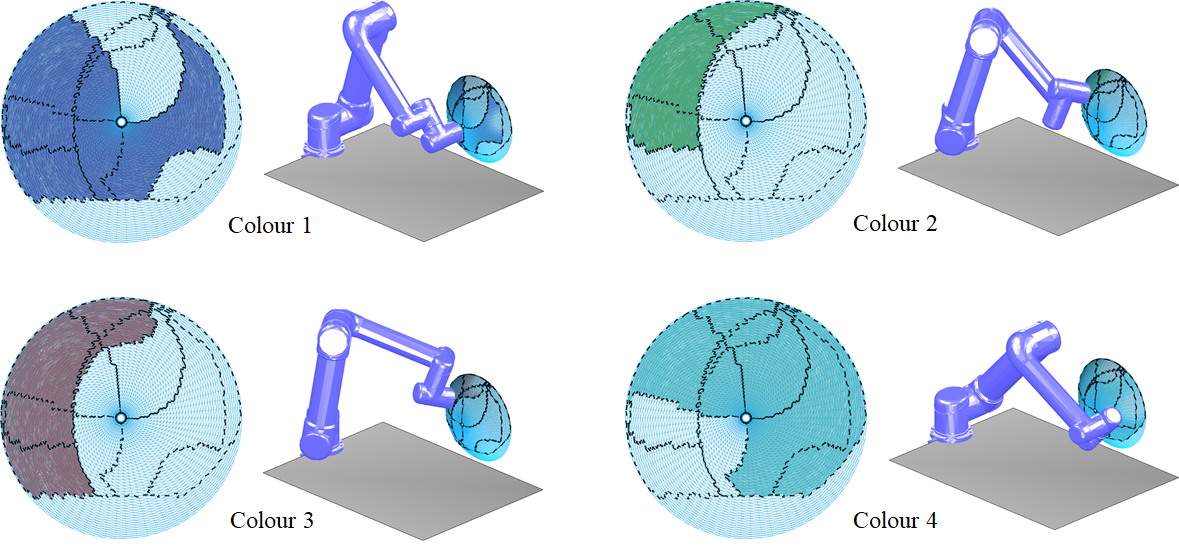
\includegraphics[width = 0.44\textwidth]{figures/exp_central_sphere/ground_truth_demo_color_2}
\caption{Illustration of the examples of available configurations, colour distributions and initial topological graph in covering part of a sphere. 
The singular point is at the center of the mesh. 
In order to visualize all valid configurations, we need the kinematic mapping to be one-to-one, so we remove showing the continuity given by the singular point. 
From the detailed explanation in Fig.~\ref{fig:bad_mesh} we know that colour $1$ and colour $4$ are joint-space continuous when considering singularities. 
%The mesh is dense, and properly designed near the singular point, so this figure can be seen as the ground truth. 
}\label{fig_ground_truth}
\end{figure}

\subsection{Counterexample of CPP in Non-complete Configuration Set}
In this subsection, we provide a counterexample that if the waypoints for CPP are not complete, then the CPP solution cannot leverage the valid singularities to avoid EE lift-offs. 
We again take the sphere as an example. 
For better illustration, we add a ground plane to remove all elbow-down configurations and leave only the central part of the mesh of the sphere. 

We first show the groundtruth solution on analytic surface, and land back to the discrete situations. 
The demo of available configurations, colour distributions and initial topological graphs are shown in Fig.~\ref{fig_ground_truth}. 
The center of the surface is the singular point, and the EE can smoothly traverse the singularity as long as the instant motion direction remains static. Hence colour $1$ and $4$ are continuous when considering the valid singularities. 
It is apparent that the optimal number of lift-off is $0$ when considering the singularity: the manipulator covers the left part using colour $1$ and then smoothly transits to colour $4$ by passing the singularity, and finally covers the right part using colour $4$. 

\begin{figure}[t]
\centering
\subfigure[IK solutions of vertices when the mesh is sparse. No path planner will regard any two configurations in the figure as continuous, because moving the EE along any of four mesh edges requires much adjustment to the manipulator pose.]{
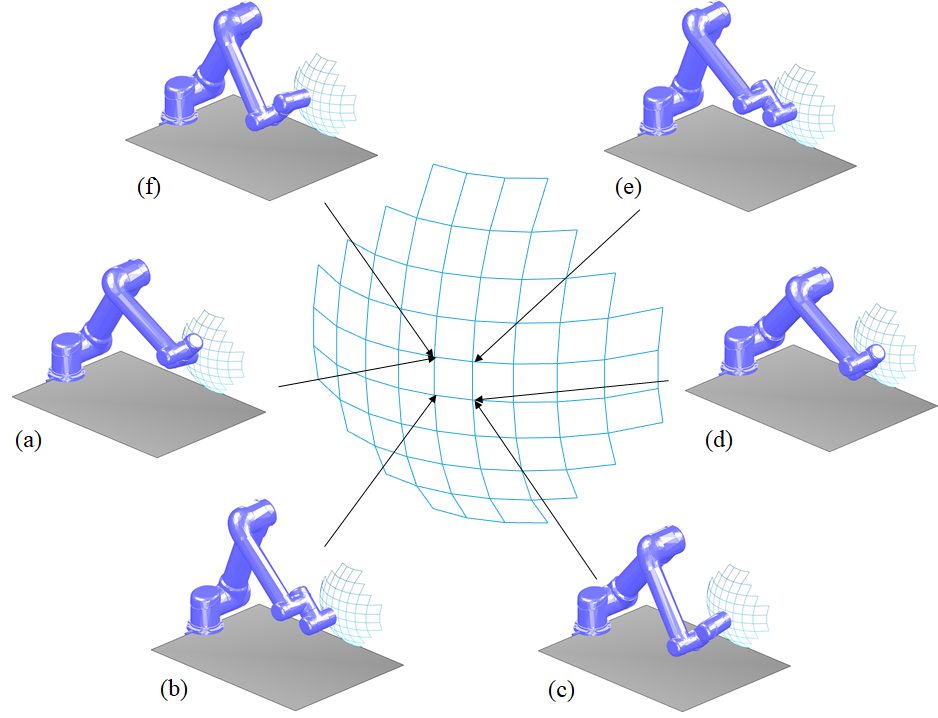
\includegraphics[width = 0.44\textwidth]{figures/exp_central_sphere/sparse_confs_2}\label{fig:nearest:a}
}
\subfigure[IK solutions of vertices after the mesh is refined. (b') and (c') are denoted as the same colour, but it does not mean that the EE can move directly from (b') to (c'). They are continuous because the configurations (g)(h) are inserted as waypoints, which makes (b) and (c) continuous. 
A direct motion from (b') and (c') has huge wrist motion which is not regarded as continuous by the path planner (denoted by a $\times$ in the enlarged figure). ]{
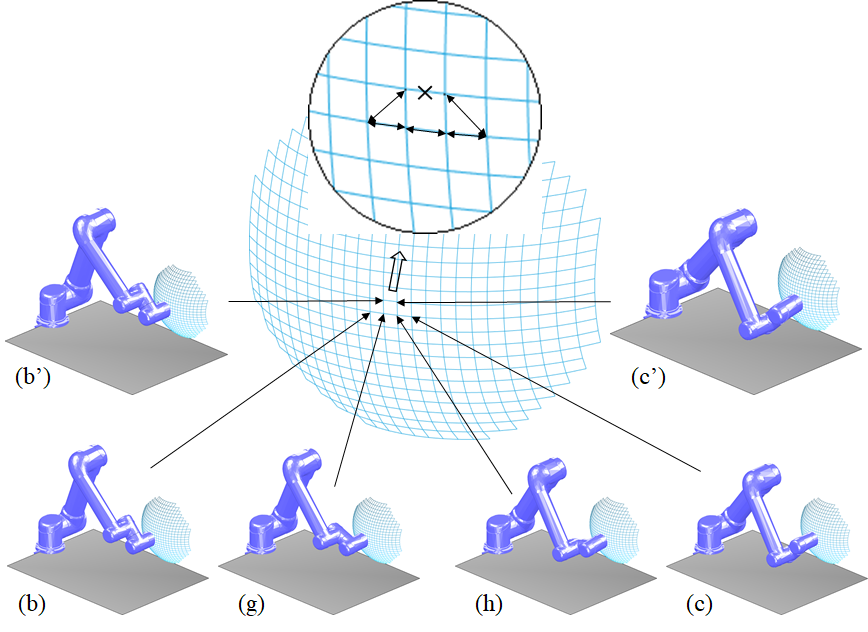
\includegraphics[width = 0.44\textwidth]{figures/exp_central_sphere/sparse_refined}\label{fig:nearest:b}
}
\caption{Illustration of how configurations are connected and how the singularity cannot be leveraged. The colour number follows the definition in Fig.~\ref{fig_ground_truth}. }\label{fig_nearest}
\end{figure}

Then it comes to the discrete situations. 
We first show how the algorithm can connect the configurations belonging to a same colour without passing singularity. For the pattern of the mesh, denote the radius of the sphere by $R$, and the surface is sampled using a planar $n\times n$ grids template, with rising of the vertices in the third dimension. I.e., we first design the vertex $p_{ij}$ on a planar grid, 
\begin{equation}
p_{ij} = \left(\frac{2i-n}{n}R, \frac{2j-n}{n}R\right), i, j = 1, \cdots, n
\end{equation}
a sampling point $\tilde{p}_{ij}$ is chosen as
\begin{equation}
\tilde{p}_{ij} \triangleq \left(\frac{2i-n}{n}R, \frac{2j-n}{n}R, \sqrt{1 - \frac{(2i-n)^2}{n^2} - \frac{(2j-n)^2}{n^2}}R\right)
\end{equation}
$n$ is set as an odd number, so that there is always no vertex that precisely represents the singular point. 
The configurations covering the four nearest vertices to the singular point are depicted in Fig.~\ref{fig:nearest:a}, where in such a sparse selection of configurations, no path planner would see them as continuous configurations. However, as the mesh is refined to Fig.~\ref{fig:nearest:b}, (a)(b)(c) are continuous (belonging to colour 1 in Fig.~\ref{fig_ground_truth}) and (d)(e)(f) are continuous (belonging to colour 4 in Fig.~\ref{fig_ground_truth}), but the new central configurations (b')(c') still have huge wrist joint angle difference thus are not considered as directly connectable by the planner. 
The configuration (b') and (c') are assigned with the same colour because the connectivity tracks (b')$\leftrightarrow$(b)$\leftrightarrow$(g)$\leftrightarrow$(h)$\leftrightarrow$(c)$\leftrightarrow$(c'). 
It can be seen that for a straight motion of EE from (b') to (c'), a non-redundant joint-space trajectory exists but, like the motion (b)$\leftrightarrow$(g)$\leftrightarrow$(h)$\leftrightarrow$(c), will have a huge wrist flipping. 
This in effect indicates that the joint-space near singularities is not flat, as such a small motion of the EE may cause a long joint-space motion. 

Now we show how configurations belonging to different colours, (b) and (d), are joint-space connectable. 
The continuous trajectory is given in Fig.~\ref{fig:bad_mesh}, where a null motion is inserted in between. 
The EE first moves to the analytic center of the central grid, then performs a null motion, and finally moves to the target configuration (d). 
With its resolution $n$ increasing, for each point on the surface, there will be a vertex of the mesh which stays arbitrarily close to it, but within the IK solutions of all vertices of the mesh the connectivity between configuration (b) and (d) cannot be observed. 
Thus this example becomes a counterexample choice of coverage waypoints, which is not asympotitally complete to leverage the singularities to avoid EE lift-offs. 

\begin{figure}[t]
\centering
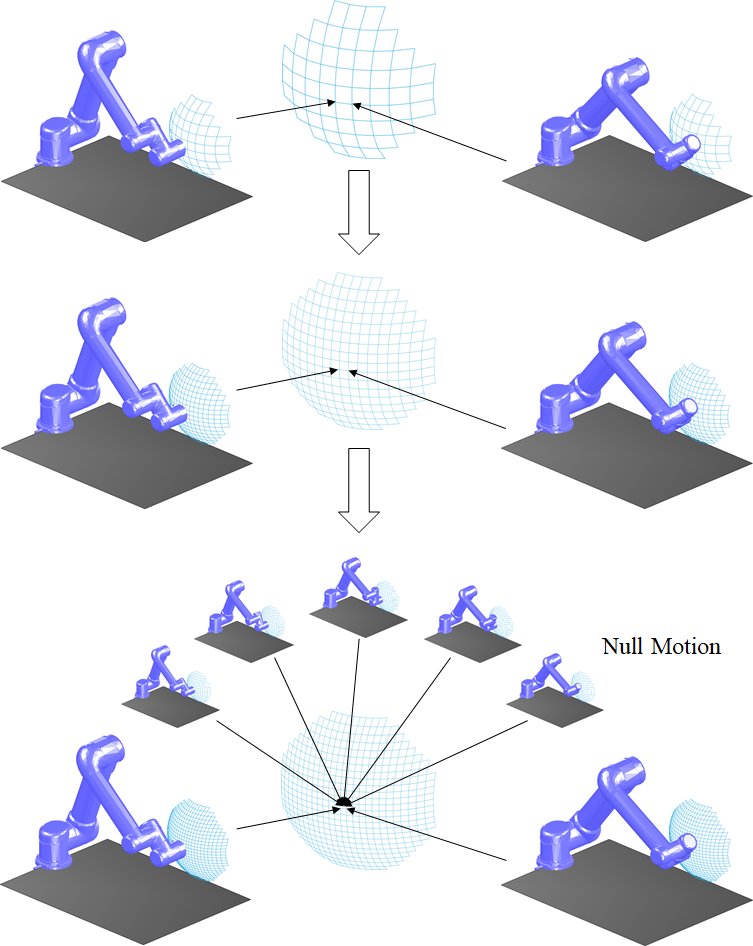
\includegraphics[width = 0.44\textwidth]{figures/exp_central_sphere/pass_to_controller}
\caption{
When the grid is refined both horizontally and vertically, the singular point is always at the center of a square. Hence no matter how precise the mesh is, it does not have a smooth transition of the singular point. }\label{fig:bad_mesh}
\end{figure}

\subsection{Practical Solution to SNCPP in Discrete Mesh}
\begin{figure}[t]
\centering
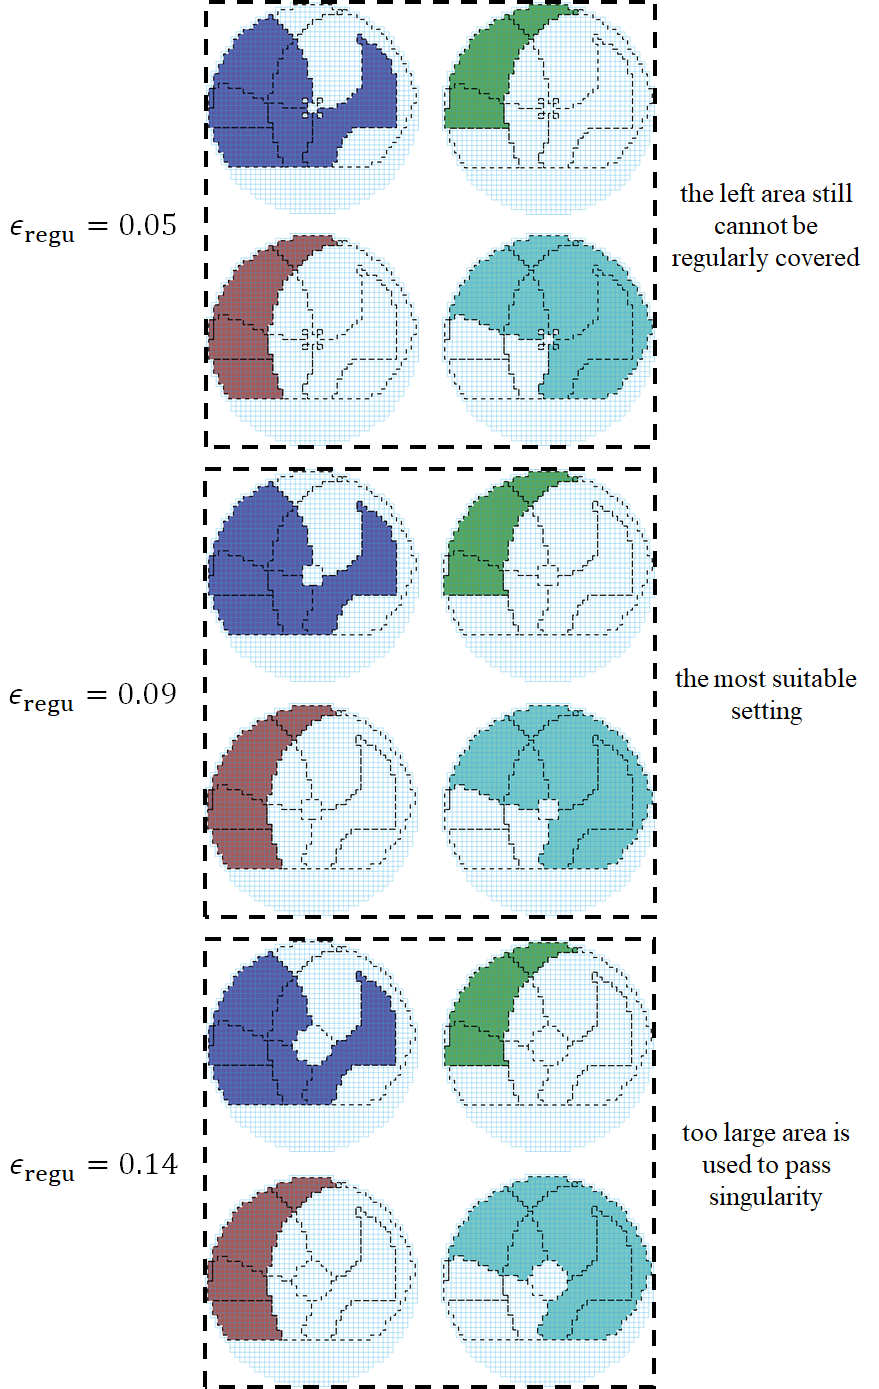
\includegraphics[width = 0.48\textwidth]{figures/exp_central_sphere/choose_threshold_2}
\caption{Illustration of different $\epsilon_{\rm regu}$ for assigning a most suitable region for passing the singularity. It depends on the configuration continuity threshold $\epsilon_{\rm cont}$. 
The joint-space near singularity is not flat, the continuity of configurations near singularity cannot be observed, leading to some configurations which are disconnectable to all configurations of its neighbouring vertices. 
$\epsilon_{\rm regu}$ is set to exclude those irregular configurations, such that other configurations can be arbitrarily connected when designing coverage paths. 
In this example, $\epsilon_{\rm regu} = 0.05$ is not enough, because there are still four configurations that cannot connect to adjacent configurations. 
$\epsilon_{\rm regu} = 0.14$ is a valid parameter, however, it splits too many configurations, reducing the region that could have been covered by coverage paths. 
In contrast to $0.05$ and $0.14$, $\epsilon_{\rm regu} = 0.09$ is a better setting. 
}\label{fig:choose_threshold}
\end{figure}

\begin{figure}[t]
\centering
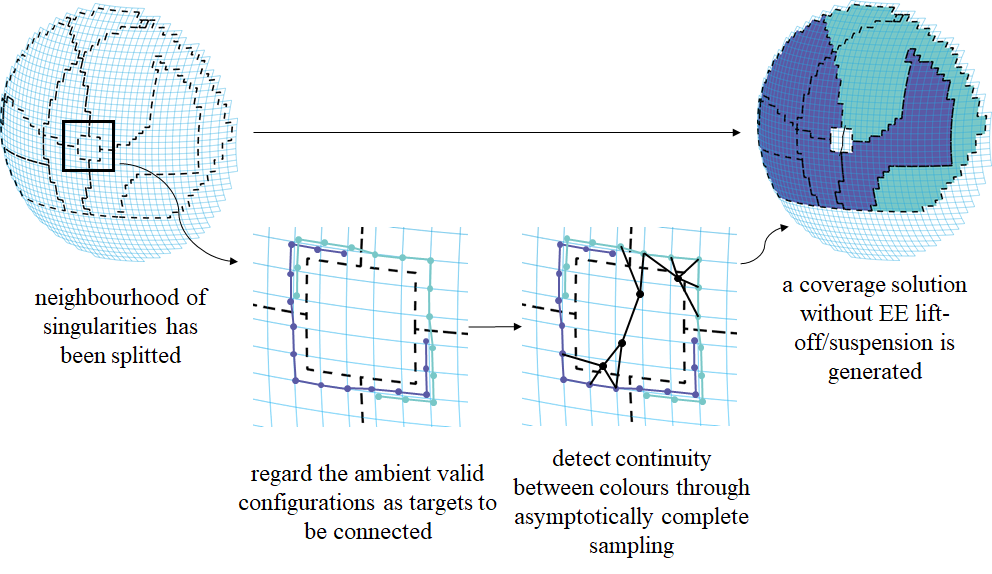
\includegraphics[width = 0.48\textwidth]{figures/exp_central_sphere/complete_sampling/complete_sampling}
\caption{Concept of asymptotically complete path finding in the splitted area. Points with different colours mean different IK solutions to cover the mesh vertices. After the black path is planned, the coverage task for this object requires $0$ EE lift-off. }\label{fig:complete_sampling}
\end{figure}

As a simple corollary to the result in Section \ref{subsection_asymptotical}, ``pure ramdom sampling of coverage waypoints with distance-based continuity" is a valid strategy asymptotically ensuring smooth transition between colours. 
However, if waypoints are not regularly sampled, such as using the curvilinear coordinates, conventional coverage path solutions cannot be easily adopted. 
Finding a non-repetitive coverage path on a random mesh is equivalent to finding a Hamilton path on the graph, an NP problem which is undesired in realistic application. 
Recall that in Section \ref{subsection_all_finiteness} we have splitted the whole surface $M$ into two parts, 
\begin{equation}
M = \tilde{M} \cup \left\{\bigcup\limits_{\lambda\in \Lambda}B(x_\lambda, \delta_{x_\lambda})\right\}
\end{equation}
where $\tilde{M}$ can be covered with full non-singular configurations, and the last term goes to infinitely small to make $\tilde{M}$ and $M$ having same surface area. 
\begin{color}{blue}
This motivates us to practically leave the joint-space area surrounding the singularity specially for leveraging the singularity. 
The size of the area is properly chosen such that all the left-out configurations are ``flat" enough that can be arbitrarily used for tracking regular template coverage paths on the surface. 

Following this idea, we extraly pick up all configurations which have manipulability less than $\epsilon_{\rm regu}$. 
For each valid singularity such as $x_\lambda$, the set of selected configurations surrounding $x_\lambda$ is denoted as $C_{x_\lambda} = \{c_{x_\lambda \gamma_\lambda}\}_{\gamma_\lambda \in \Gamma_\lambda}$. $C_{x_\lambda}$ will cover a piece of task-space region $M_{x_\lambda}$ on the surface. 
$\epsilon_{\rm regu}$ should be chosen big enough to include all valid, non-singular but ``unflat" configurations such that, outside $M_{x_\lambda}$ one can arbitrarily design the coverage path, ensuring a continuous joint-space path outside $C_{x_\lambda}$. 
Within the $\epsilon_{\rm regu}$-neighbourhood of the valid singularity, we try obtaining connectivities of the surrounding non-singular configurations outside the neighbourhood. 
From another perspective, $\epsilon_{\rm regu}$ cannot be too big because too large $M_{x_\lambda}$ might be preserved for transition to singularity which damages the performance of the coverage task.  
See Fig.~\ref{fig:choose_threshold} for an illustration of the choice of $\epsilon_{\rm regu}$. 
For obtaining the connectivities in $C_{x_\lambda}$ visiting the singularity, they are easy to get, because theoretically the configurations to be connected stay symmetrically to the singularity. 
\end{color}
See a concept map in Fig.~\ref{fig:complete_sampling}. 
Sampling-based planners (such as the RRT*~\cite{Karaman2011Sampling} algorithm) can be adopted for probabilistically complete path planning and we omit further description. 
Note that it is not our focus to finding the optimal parameter $\epsilon_{\rm regu}$ for a concrete object, or choosing different optimal parameters for different singularities on the object. 
We concentrate on how to simultaneously applying conventional solutions for the CPP task and leveraging the valid singularities, and the proposed strategy works for this. 

\textcolor{red}{TODO: Do we need an algorithmic block ?}

%\subsection{Summary}
%In Section \ref{section_analytic} and \ref{section_discrete} we face with the problem of adapting valid singular configurations in the SNCPP problem, which makes the mapping from valid configurations to task space regions to be non-bijective, and the coverage path in cells becoming non-arbirarily designed. 
%Seeing that the singularities only form zero-area region, we prove the finiteness of cells in the graph. We prove that the transition between colours on the surface is applicable when passing singularities, and a non-stopping smooth EE motion can be established if it goes in the permissible direction when passing singular point. 
%For discretely represented surface meshes, we propose necessary and sufficient condition for the waypoints selection to implicitly pass the singularities without a mesh vertex staying exactly on the singular point. A practical method is proposed to simultaneously leverage singularities and template coverage paths.  
%
%Eventually, even if the colours in the SNCPP problem becomes non-bijective, the problem can still be completely separated into two independent stages, the optimal cellular decomposition stage and the coverage path designing and tracking stage. 
%Hence the solution of the SNCPP problem can still land back to discussion on solving all kinds of topological graphs.

%\begin{table}[t]
%\small\sf\centering
%\caption{UR5 Manipulator Kinematic Parameters}\label{table:ur5_kinematics}
%\begin{tabular}{>{\bfseries}lllll}
%\toprule
%\normalfont{Joint i}   &     $\bm{\alpha_i}$ [rad]    &   $\bm{a_i}$  [m]    &    $\bm{\theta_i }$ [rad]   &    $\bm{d_i}$  [m]   \\
%\midrule
%1 & $\pi/2$ & 0 & $\theta_1$ & 0.089 \\
%2 & 0 & $-0.425$ & $\theta_2$ & 0 \\
%3 & 0 & $-0.39225$ & $\theta_3$ & 0 \\
%4 & $\pi/2$ & $0$ & $\theta_4$ & 0.11 \\
%5 & $-\pi/2$ & 0 & $\theta_5$ & 0.09 \\
%EE & $0$ & 0 & - & 0.32\\
%\bottomrule
%\end{tabular}
%\end{table}


\begin{color}{blue}

\section{Experimental Results}\label{section_exp}
Several representative simulation works have been implemented to validate the proposed algorithm on challenging arbitrarily-shaped objects. 
We use a typical 6 DoF manipulator, a Universial Robots UR5. 
%The kinematics of the manipulator are collected in Table \ref{table:ur5_kinematics}. 
For such endeavour, the (commonplace) final revolute joint of the manipulator is unnecessary given the rotating nature of the polishing tool itself. This is indeed the case for the UR5, and simulations and real evaluation have thus been undertaken where the lask link has been locked. 
\end{color}

\begin{figure}[t]
\centering
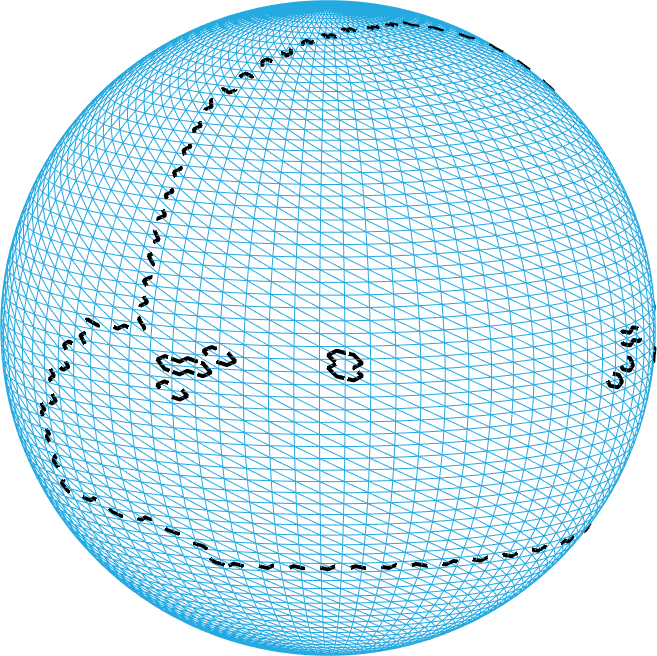
\includegraphics[width = 0.24\textwidth]{figures/real_world/whole_graph_left}
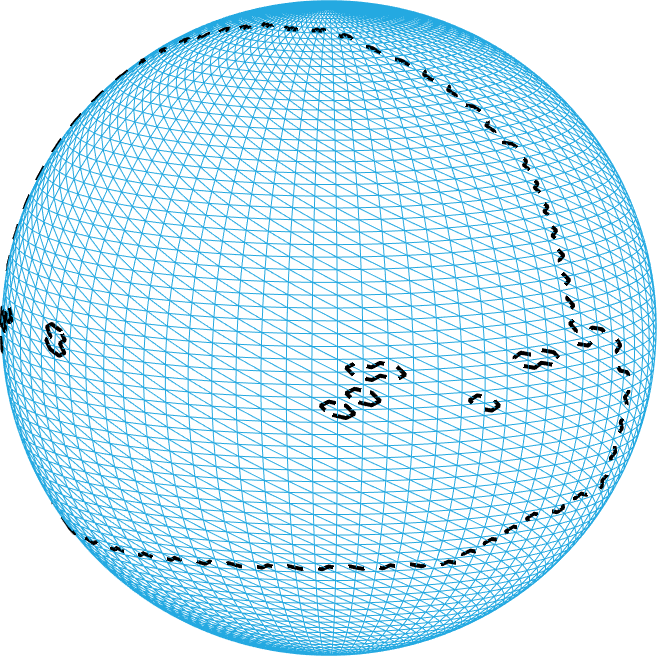
\includegraphics[width = 0.24\textwidth]{figures/real_world/whole_graph_right}
\caption{The initial topological graph without splitting a neighbourhood area surrounding valid singularities. 
Multiple IK solutions are observed to be assigned the same colour, which breaks the definition of initial topological graphs and indicates the existence of colour connectivities given by valid singularities. }\label{fig:whole_graph}
\end{figure}


\begin{figure}[t]
\centering
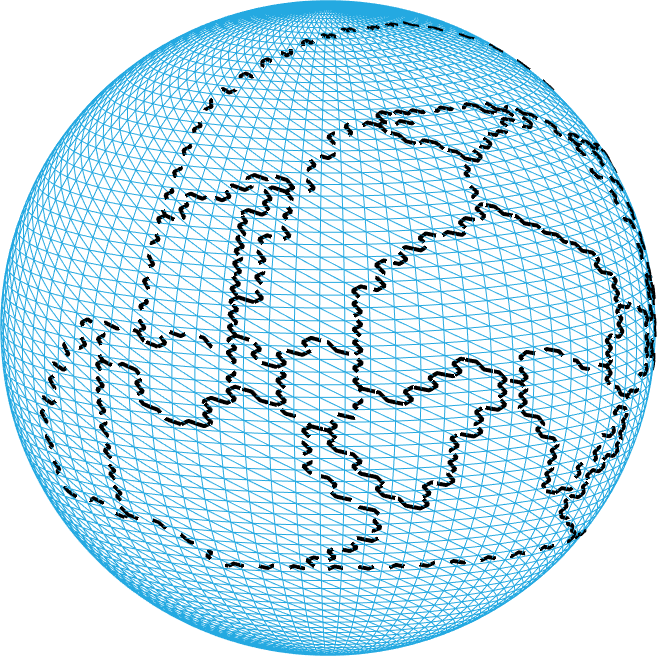
\includegraphics[width = 0.24\textwidth]{figures/real_world/init_graph_left}
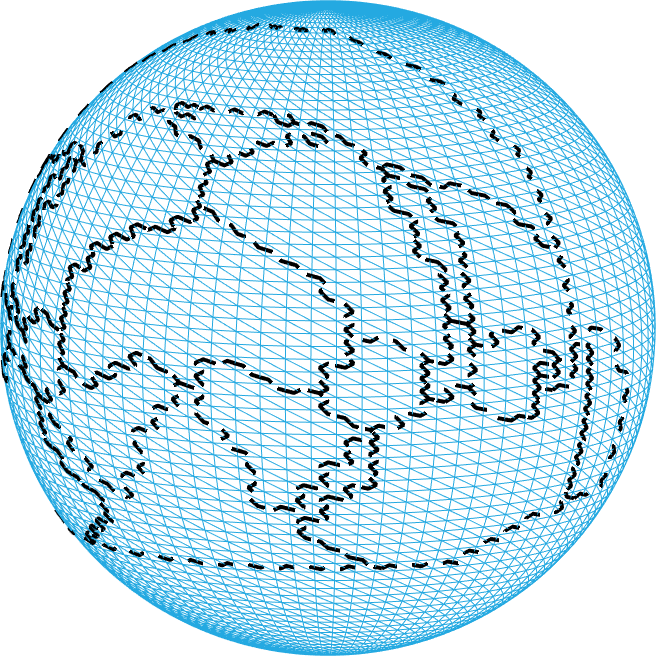
\includegraphics[width = 0.24\textwidth]{figures/real_world/init_graph_right}
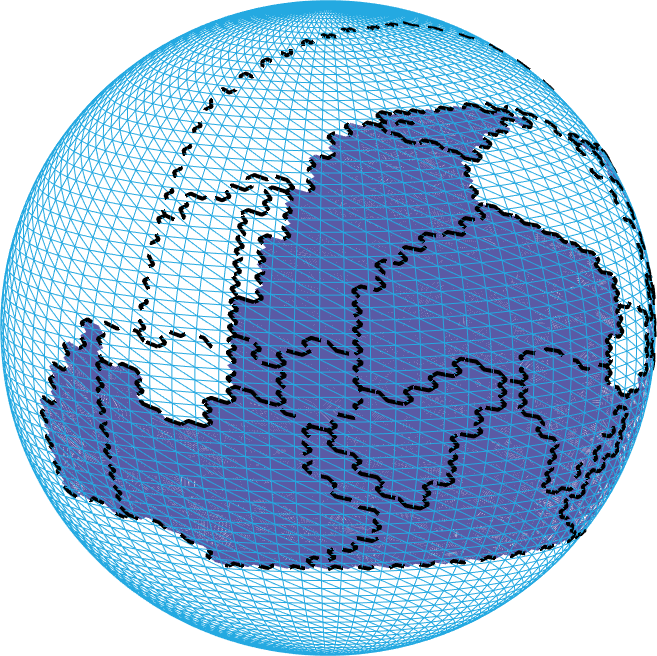
\includegraphics[width = 0.24\textwidth]{figures/real_world/color_1_left}
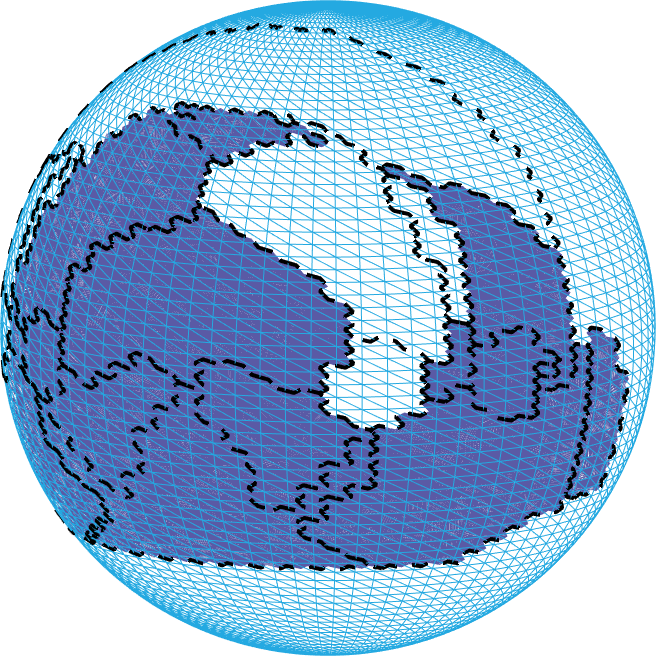
\includegraphics[width = 0.24\textwidth]{figures/real_world/color_1_right}
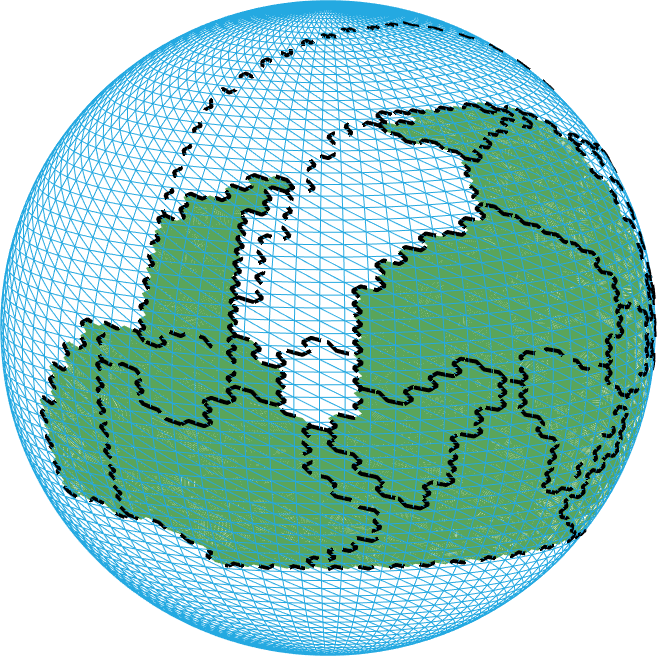
\includegraphics[width = 0.24\textwidth]{figures/real_world/color_2_left}
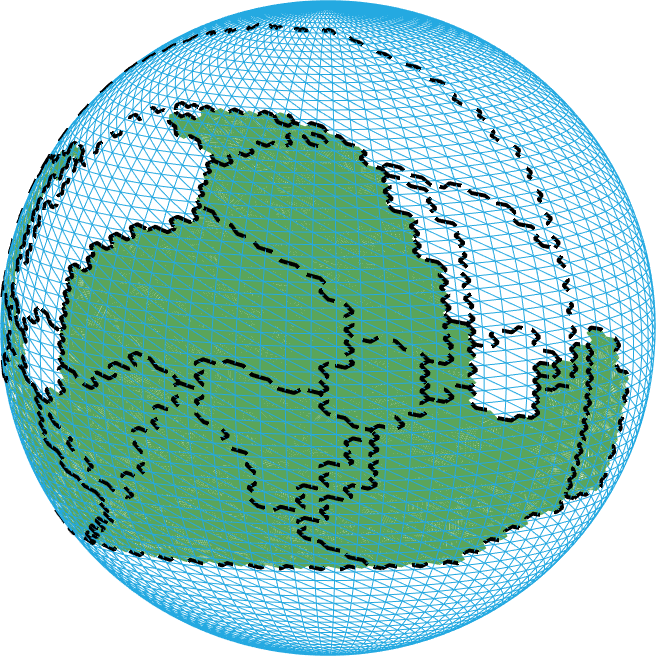
\includegraphics[width = 0.24\textwidth]{figures/real_world/color_2_right}
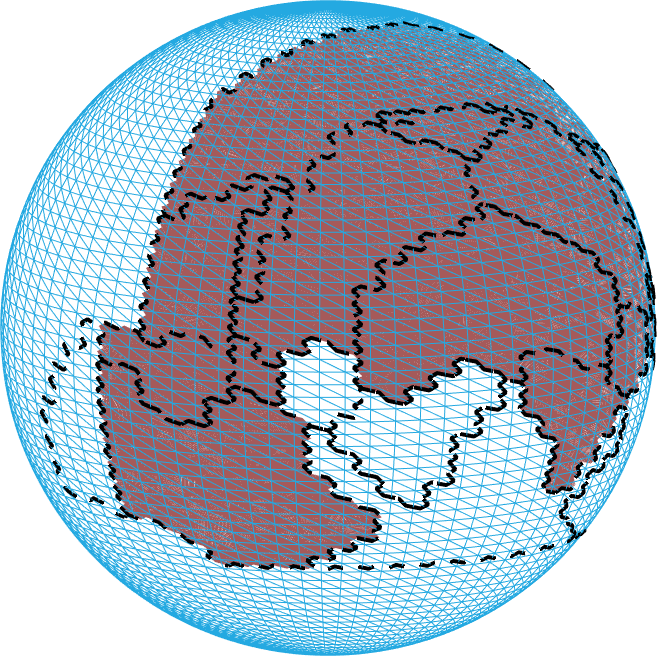
\includegraphics[width = 0.24\textwidth]{figures/real_world/color_3_left}
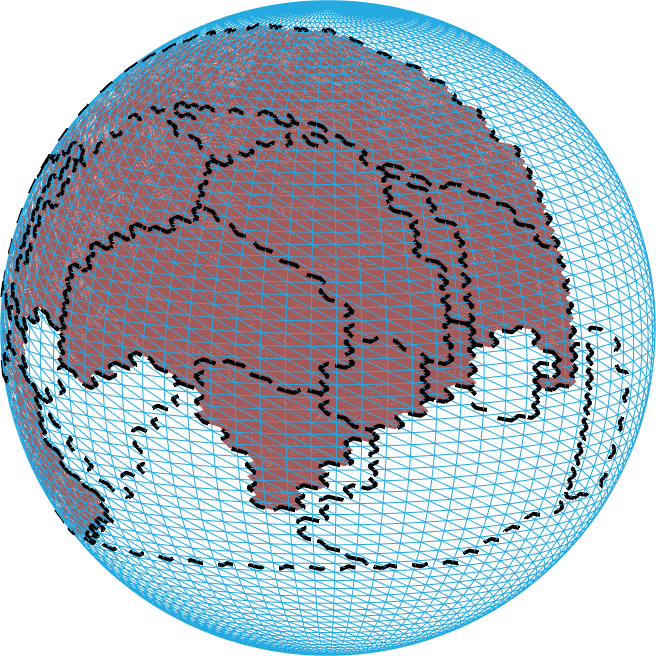
\includegraphics[width = 0.24\textwidth]{figures/real_world/color_3_right}
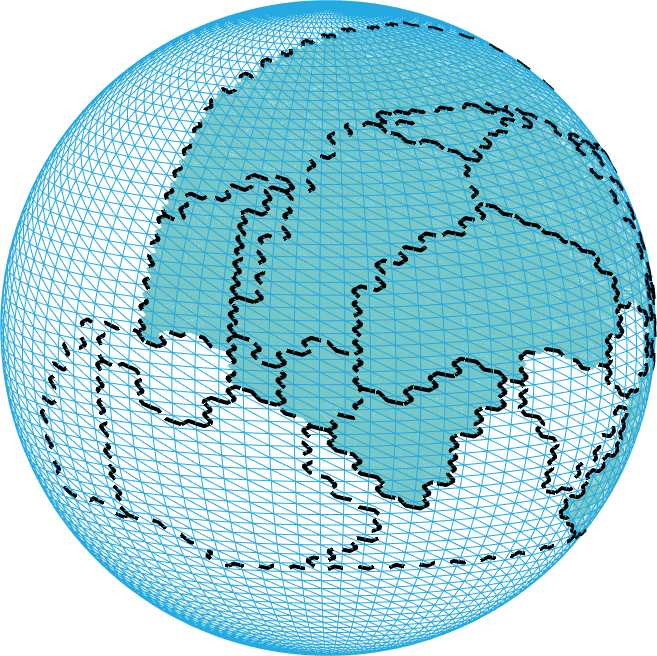
\includegraphics[width = 0.24\textwidth]{figures/real_world/color_4_left}
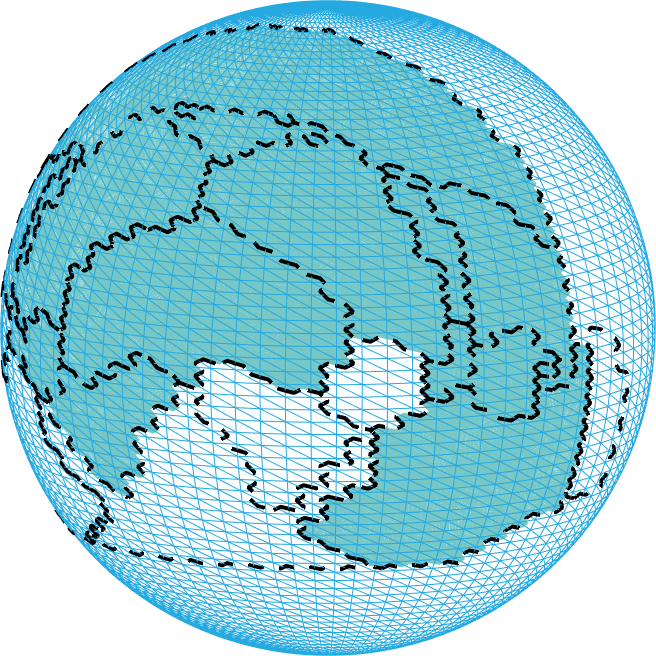
\includegraphics[width = 0.24\textwidth]{figures/real_world/color_4_right}
\caption{Illustration of the topological graph and reachable area of colours after remove the neighbourhood of singularities. Each continuous set of valid configurations is injective to the surface points}\label{fig:bijective_graph}
\end{figure}

\begin{figure*}[t]
\centering
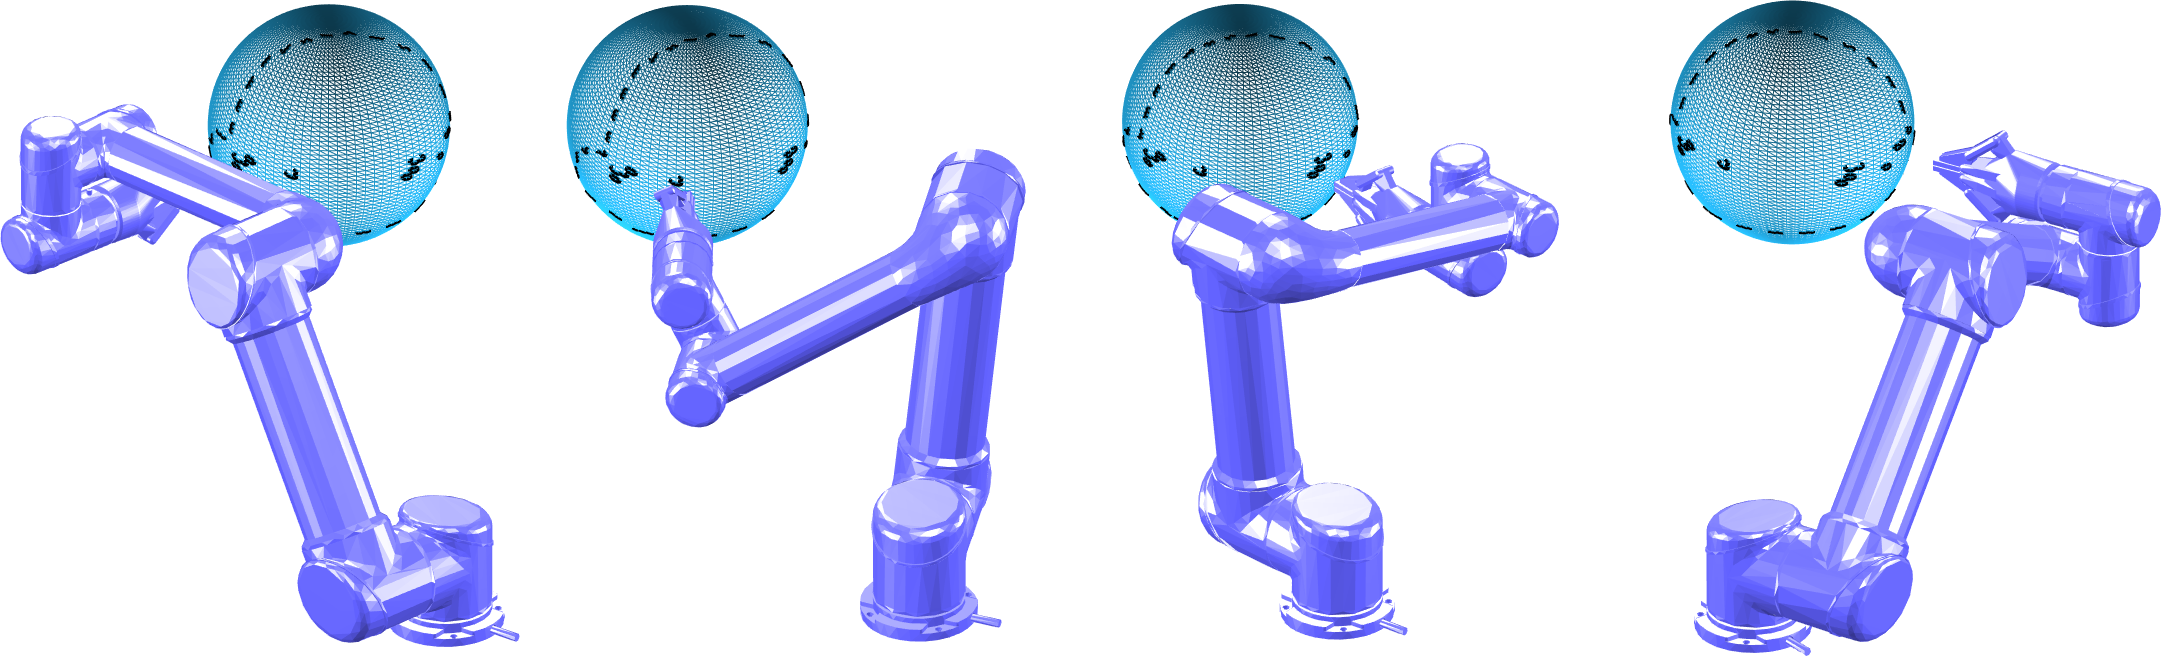
\includegraphics[width = 0.96\textwidth]{figures/real_world/pose_comb}
\caption{Illustration of four non-singular configurations which are very near a singularities. Indexing the singularity from left to right, it is apparent to see that the singularity $1$ and $3$ are caused by the shoulder-left configurations, while $2$ and $4$ are caused by the shoulder-right configurations.}
\end{figure*}

\begin{color}{red}
\subsection{Simulated Evaluation}\label{subsection_simulated}

\subsection{Real-World Experiments}\label{subsection_realworld}

Finally, we show a real-world covering task of a spherical object, together with detailed process of simultaneously leveraging singularities and template coverage paths. For the simplicity of description, other irrelavant configurations (colours) are omitted. 
The initial topological graph when directly running the algorithm is shown in Fig.~\ref{fig:whole_graph}. The whole region is almost in a same cell (together with some isolated configurations that are given different colours), which reveals a $0$ lift-off solution of the coverage task. However, the available colour of the cell does not uniquely corresponds to an IK solution, and some single configurations are given different colours than its neighbours, which indicate the existence of singularities. Direct trials of boustrophedon path fail unsurprisingly. 
After removing the vicinity of singularities following the criterion in Equ.~(\ref{equ_remove_neighbour}), a new topological graph appears with all colours being bijective between the joint-space and the surface points, shown in Fig.~\ref{fig:bijective_graph}. From the removed configurations we know that there are four singularities. Indexing the singularities visually from left to right, $1$ and $3$ are actually caused by the shoulder-left configurations, and $2$ and $4$ are caused by the shoulder-right configurations. Thus no matter which pair of connectable colours we choose, two singular points are actually not singular and can be covered with regular coverage path, whilst one of the other two singularities is used to do smooth manipulator pose adjustment. 
In our case, we use the configurations corresponding to the green colour and the red color, together with a smooth transition passing singularity $2$. The proposed algorithm is able to come up with an effective solution with no EE lift-off or suspension. The reader is referred to the associated video for demonstration. 


\begin{figure*}[t]
\centering
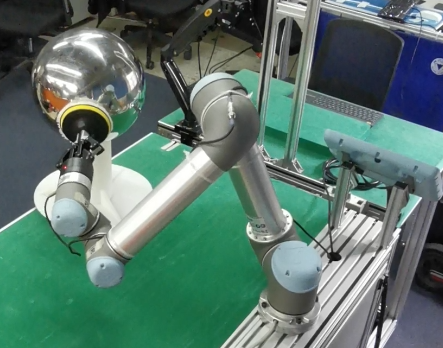
\includegraphics[width = 0.19\textwidth]{figures/real_world/show_huge_change/pose_1}
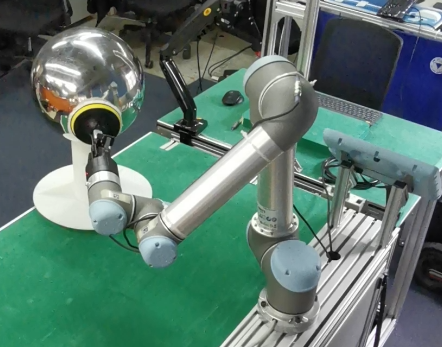
\includegraphics[width = 0.19\textwidth]{figures/real_world/show_huge_change/pose_2}
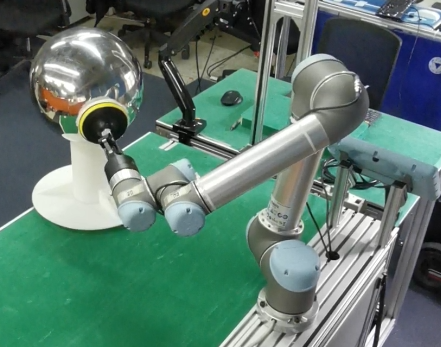
\includegraphics[width = 0.19\textwidth]{figures/real_world/show_huge_change/pose_3}
\includegraphics[width = 0.19\textwidth]{figures/real_world/show_huge_change/pose_4}
\includegraphics[width = 0.19\textwidth]{figures/real_world/show_huge_change/pose_5}
\caption{Illustration of a manipulator motion near the singularity. While the EE pose does not change much, the wrist rotates for almost $\pi$ rad. }\label{fig:boust}
\end{figure*}

In contrast to the proposed algorithm, we also show that boustrophedon path is not applicable given the severe pose changes of the manipulator near the singularity. See Fig.~\ref{fig:boust} for a clip of motion near the singularity. Although the EE pose does not change much, the wrist rotates almost $\pi$ rad, from below the EE to above the EE. As one could expect that when the EE is passing the singularity, it itself will not move any more and only the wrist is moving, leading to EE suspension at the singular point. 

Moreover, the spiral path are neither applicable, because except within the vicinity of the singularity, the configurations belonging to different colours are not continuous. See Fig.~\ref{fig:two_points} for the visualization of two configurations belonging to different colours. They are indeedly used in the final solution of the proposed algorithm, but it is obviously that direct concatenation of such configurations is not continuous (a jump from wrist-below pose to wrist-above pose is impossible). 

\begin{figure}[t]
\centering
\includegraphics[width = 0.24\textwidth]{figures/real_world/show_demo_of_two_colours/demo_2}
\includegraphics[width = 0.24\textwidth]{figures/real_world/show_demo_of_two_colours/demo_3}
\caption{These two points on the surface which are being covered would be continuously visited if we adapted pure boustrophedon path or pure spiral path, which are obviously impossible. }\label{fig:two_points}
\end{figure}
\end{color}

\begin{color}{blue}
\section{Conclusion and Future Work}\label{section_conclusion}
This paper has proposed a novel mechanism to deal with valid singular configurations during a manipulator non-revisiting coverage path planning (NCPP) task. 
Due to the existence of valid singularities, such as an elbow-straight pose, which bridge different kinds of non-singular configurations, such as the elbow-up and elbow-down poses, the number of necessary end-effector lift-offs on the surface may be further reduced, whilst the forward kinematics from each connected set of valid configurations to object surface becomes non-bijective, making existing modelling of the NCPP problem~\cite{Yang2020Cellular}~\cite{Yang2020Nonrevisiting} inapplicable. 

By carefully examining the distribution of singularities of the non-redundant manipulator, the NCPP problem with modelled to a topological graph with singularity-specified joint-space connectivities between disjointed sets of valid non-singular configurations, which has been proven finitely solvable. 
Challenging simulated comparisons and real-world evaulations supplemented by a video are provided to validate the proposed scheme.
\end{color}

\section*{Acknowledgement}
This work was supported by National Key R\&D Program of China (2018YFB1309300) National Nature Science Foundation of China (61903332, U1609210).

\appendix
\section{Solution to Topological Graph}
\subsection{Solution to Graph Consisting of Simply-Connected Cells}

\begin{color}{blue}
Respecting the definition of cells, edges, and graphs in Section~\ref{section_problem_modelling}, 
in earlier work~\cite{Yang2020Cellular}, under the assumption of all simply-connected cells, the topological graph for optimal NCPP was solved in an exhaustive manner, which is essentially an optimal design strategy of a colour (configuration) scheme whereby the strategic placement of cutting paths would invariably lead to different colour vertices on both sides of a partition. Three kind of equivalent cell sub-divisions have been observed, which were safely disregarded during enumeration: 
\begin{enumerate}
\item Cutting paths which start or and at a point other than an endpoint of an edge are unnecessary. 
\item Cutting paths which go across any edge are unnecessary. 
\item Intersected cutting paths are unnecessary. 
\end{enumerate}

As a result, the remaining number of different cell sub-divisions was shown to be finite, and the graph painting problem can be enumeratively solved by iteratively dividing and painting all cells. 

\subsection{Solution to Graph Containing Multiply-Connected Cells}
To deal with the multiply-connected cells in a graph to be solved, the topology of multiply-connected cells has to be observed. 
It was noted that~\cite{Simmons1964Introduction} planar regions can be classified into different categories through their genus, i.e., the number of holes within the outer boundary. 
A genus-$n$ has $(n+1)$ boundaries (one outer boundary and $n$ inner ones), and a cutting path connecting two boundaries will transform the genus-$n$ cell to a genus-$(n-1)$ one. 
So in order to cover all situations of cells appeared in realistic application, an iterative enumeration transforming a genus-$n$ cell to sub-cells with genus no more than $(n-1)$ was motivated~\cite{Yang2020Nonrevisiting}. 
Following claims have guaranteed the finiteness of all possible different cell sub-divisions of a multiply-connected cells: 
\begin{enumerate}
\item If an inner boundary is not connected by cutting paths, then it can be temporarily removed during the solving process, and then arbitrarily placed in the solved graph. 
\item The outer boundary and the inner boundaries are equivalent when carrying out cell sub-divisions. 
\item Cyclic cutting paths will create different cellular decompositions but have the same number of end-effector lift-offs as the solution given by the acyclic cutting paths. So all cyclic cutting paths can be safely disregarded. 
\item Generating one cutting path to reduce the genus of the cell will always become a contradiction since both sides of the cutting path are effectively the same cell. Thus it is not the cutting paths but the connected area what determines the division of the multiply-connected cells. 
\item For any valid cell sub-division transforming a genus-$1$ cell to a simply-connected cell, it can be seen as a two-stage process, where two cutting paths are firstly required, and other cutting paths are designed in the resulting simply-connected sub-cells. There are finitely number of different solutions in the first stage, and the sub-division for simply-connected sub-cells is also finite, so genus-$1$ cells can be finitely solved. 
\item For a genus-$n$ cell, the whole cell sub-division can be seen as an $(n+1)$-stage process. At each stage, one inner part is put into one of the simply-connected sub-cells (the chosen one becomes a genus-$1$ sub-cell), and two new cutting paths are created in this sub-cell to transform it again into two simply-connected sub-cells. After $n$-stages, the genus-$n$ cell is divided into $(n+1)$ simply-connected sub-cells. 
In the final stage each sub-cell may be further divided to form all different solutions. 
The overall procedure is proven in finite steps by induction.  
\end{enumerate}
\end{color}

\bibliographystyle{plainnat}
\bibliography{IJRR21}

\vfill


%\begin{thebibliography}{99}
%\bibitem[Kopka and Daly(2003)]{R1}
%Kopka~H and Daly~PW (2003) \textit{A Guide to \LaTeX}, 4th~edn.
%Addison-Wesley.
%
%\bibitem[Lamport(1994)]{R2}
%Lamport~L (1994) \textit{\LaTeX: a Document Preparation System},
%2nd~edn. Addison-Wesley.
%
%\bibitem[Mittelbach and Goossens(2004)]{R3}
%Mittelbach~F and Goossens~M (2004) \textit{The \LaTeX\ Companion},
%2nd~edn. Addison-Wesley.
%
%\end{thebibliography}

\end{document}
